\documentclass[authoryear, 12pt]{elsarticle}

\usepackage{graphicx}
\usepackage{lineno}
\usepackage{amssymb}
\usepackage{wrapfig}
\usepackage{subfig}
\usepackage{tipa}
\usepackage{float}
\usepackage{longtable}
\usepackage[section]{placeins}
\usepackage{rotating}

%\linespread{2}
\journal{}

\begin{document}
\begin{center}
\Large
\textbf{Supplementary Materials}
\end{center}

\appendix
\renewcommand{\appendixname}{Material}

\section{Permutation Analyses}
\label{sec:permutation}
\setcounter{figure}{0}
\setcounter{table}{0}
\normalsize
How can we be sure that our primary dependent measure (anticipatory gaze switching) actually relates to turn transitions? Even if children were gazing back and forth randomly during the experiment, we would have still captured some false hits---switches that ended up in the turn-transition windows by chance.

We estimated the baseline probability of making an anticipatory switch by randomly permuting the placement of the transition windows within each stimulus (Main paper; Figure 4). We then used the switch identification procedure from Experiments 1 and 2 to find out how often participants made ``anticipatory'' switches within these randomly permuted windows. This procedure de-links participants' gaze data from turn structure by randomly re-assigning the onset time of each turn-transition in each permutation. We created 5,000 of these permutations for each experiment to get an anticipatory switch baselines over all possible starting points.

Importantly, the randomized windows were not allowed to overlap with each other, keeping true to the original stimuli. We also made sure that the properties of each turn transition stayed constant across permutations. So, while ``transition window A'' might start 2 seconds into Random Permutation 1 and 17 seconds into Random Permutation 2, it maintained the same prior speaker identity, transition type, gap duration, language condition, etc., across both permutations.

We then re-ran the statistical models from the original data on each of the random permutations, e.g., using Experiment 1's original model structure to analyze the anticipatory switches from each random permutation of the Experiment 1 looking data. We could then calculate the proportion of random data \textit{z}-values exceeded by the original \textit{z}-value for each predictor. We used the absolute value of all \textit{z}-values to conduct a two-tailed test. If the original effect of a predictor exceeded 95\% of the random model effects for that same predictor, we deemed that predictor's effect to be significantly different from the random baseline (i.e., \textit{p}$<$.05).

\newpage

For example, children's ``language condition'' effect from Experiment 1 had a \textit{z}-value of $|$3.65$|$, which is greater than 99.3\% of all $|$\textit{z}-value$|$ estimates from Experiment 1's random permutation models (i.e., \textit{p}$=$.007). It is therefore highly unlikely that the effect of language condition in the original model came from random gaze shifting.

We used this procedure to derive the random-baseline comparison values in the main text (above). However, we ran into two issues along the way: first, we had to report \textit{z}-values rather than beta estimates of each effect. Second, we had to exclude a substantial portion of the models, especially in Experiment 2 because of model non-convergence. We address each of these issues below.

\subsection{Beta, standard error, and z estimates}
We reported \textit{z}-values in the main text rather than beta estimates because the standard errors in the randomly permuted data models were much higher than for the original data. The distributions for each predictor's beta estimate, standard error, and \textit{z}-value for adults and children in each experiment are shown in the graphs below (Figures \ref{fig:E1-ChiTs}--\ref{fig:E2-AduSEs}). In each plot, the gray dots represent the absolute value of the 5,000 randomly permuted model estimates for the estimate type plotted (beta, standard error, or \textit{z}), the white circles represent the model estimates from the original data, and the black triangles represent the 95th percentile for each random distribution.

\begin{sidewaysfigure}[!htb]
  \centering
  \textbf{Experiment 1: \textit{z}-value estimates}\par\medskip
  \subfloat[Children]{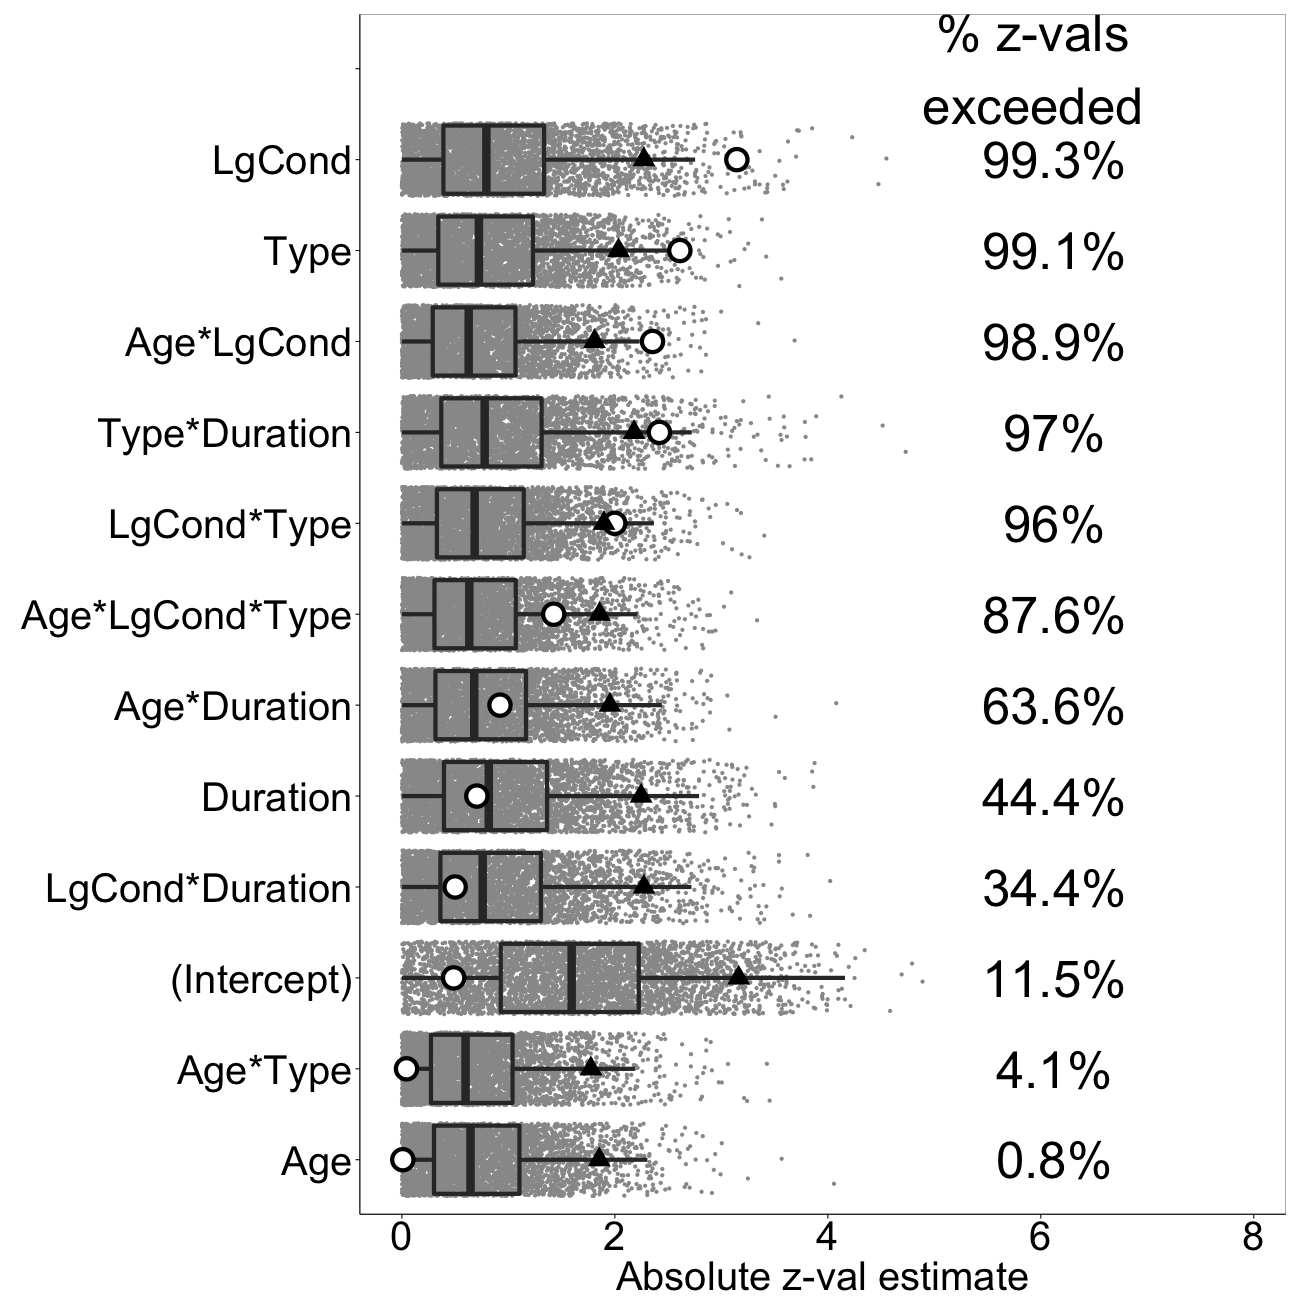
\includegraphics[width=0.44\textwidth]{figures/E1-chi-randrun-z-vals-absolute.png}\label{fig:E1-ChiTs}}
  \hfill
  \subfloat[Adults]{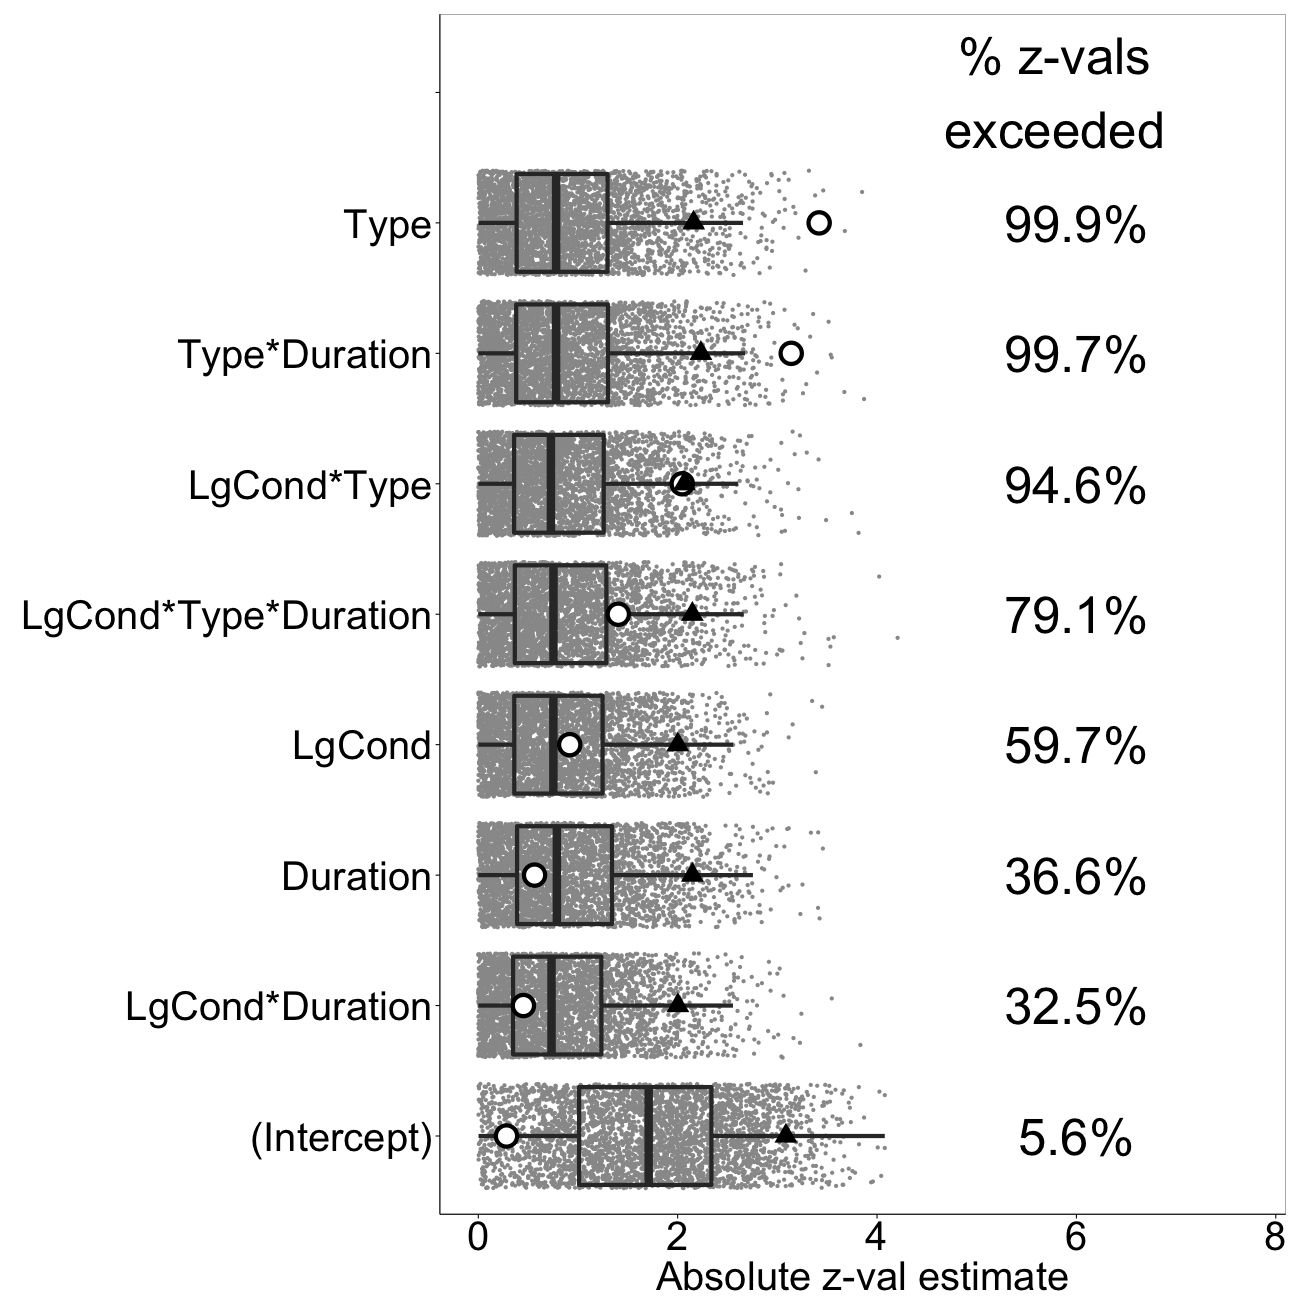
\includegraphics[width=0.44\textwidth]{figures/E1-adu-randrun-z-vals-absolute.png}\label{fig:E1-AduTs}}
  \caption{Random-permutation and original $|$\textit{z}-values$|$ for predictors of anticipatory gaze rates in Experiment 1.}
\label{fig:E1-Ts}
\end{sidewaysfigure}

\begin{sidewaysfigure}[!htb]
  \centering
  \textbf{Experiment 1: \textit{$\beta$} estimates}\par\medskip
  \subfloat[Children]{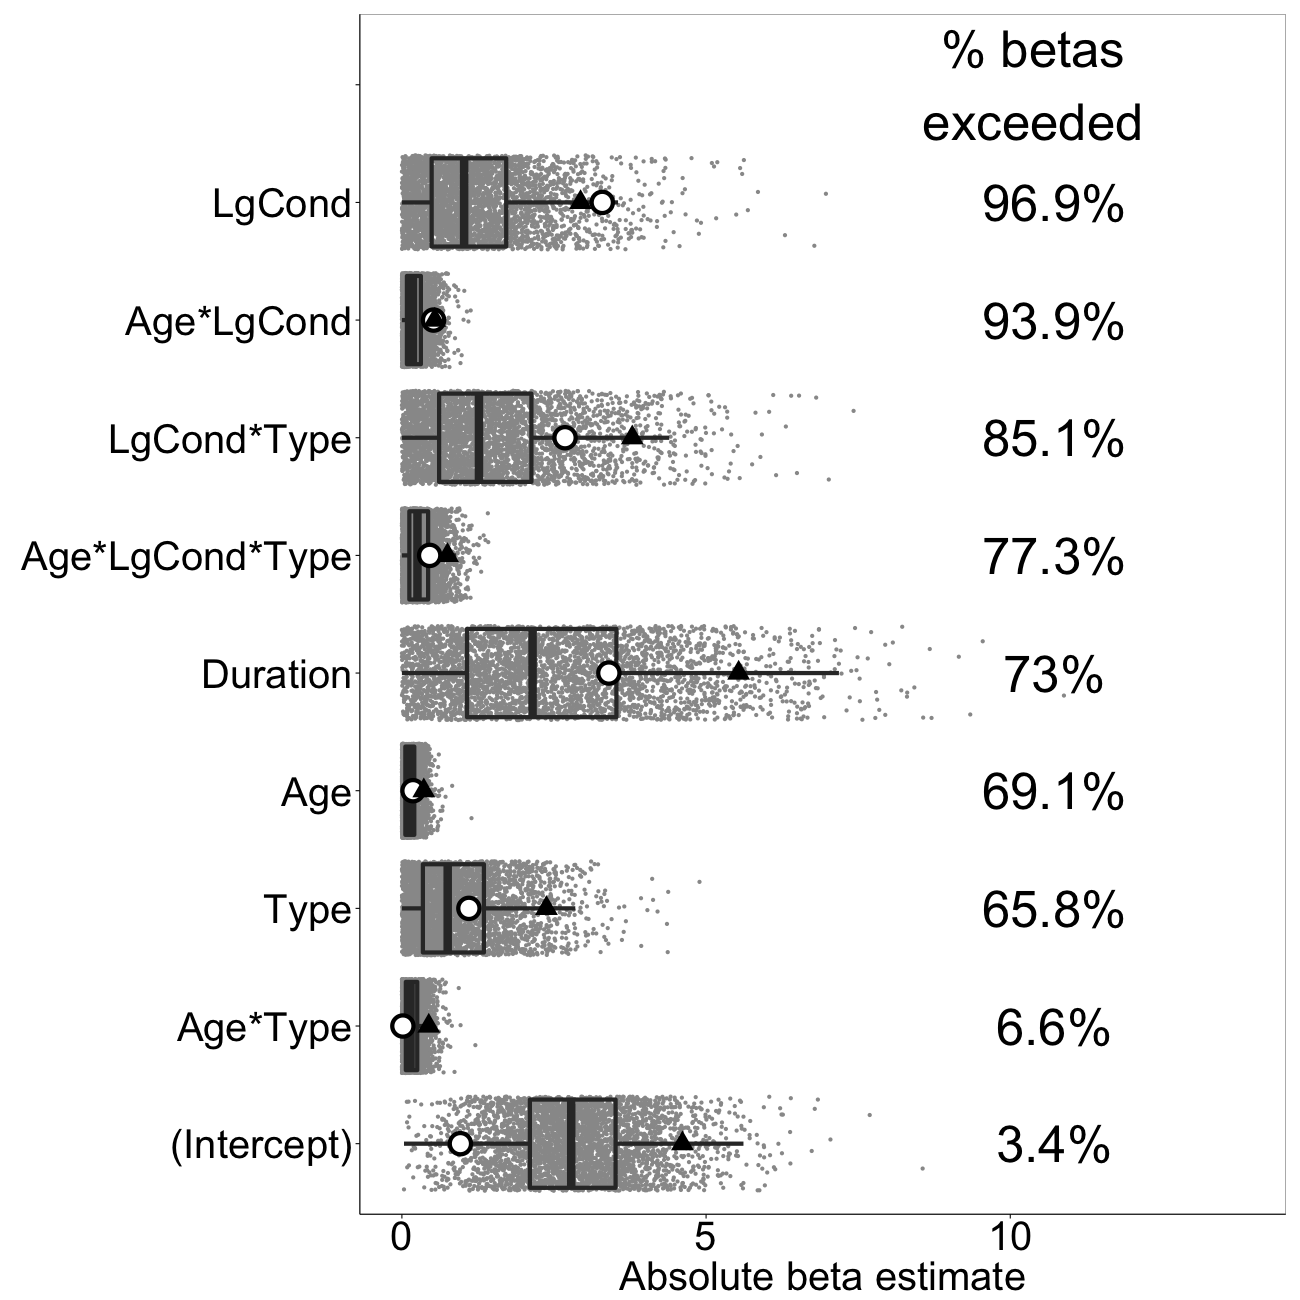
\includegraphics[width=0.44\textwidth]{figures/E1-chi-randrun-betas-absolute.png}\label{fig:E1-ChiBs}}
  \hfill
  \subfloat[Adults]{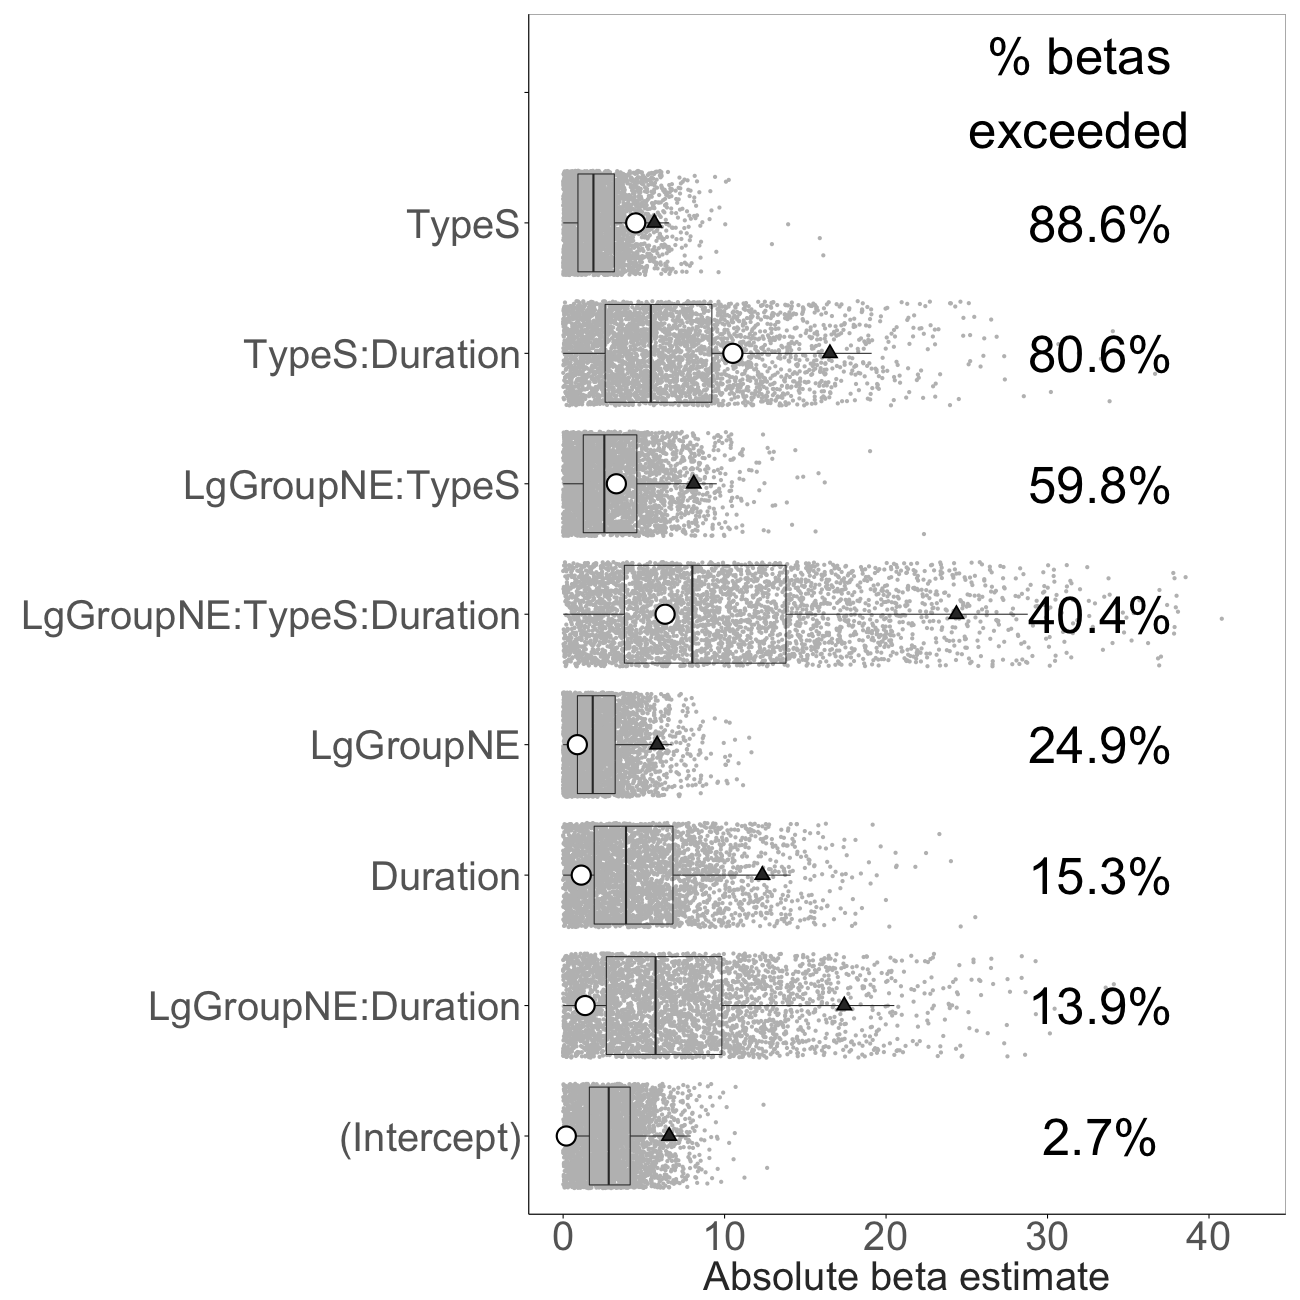
\includegraphics[width=0.44\textwidth]{figures/E1-adu-randrun-betas-absolute.png}\label{fig:E1-AduBs}}
  \caption{Random-permutation and original $|$\textit{$\beta$}-values$|$ for predictors of gaze rates in Experiment 1.}
\label{fig:E1-Bs}
\end{sidewaysfigure}

\begin{sidewaysfigure}[!htb]
  \centering
  \textbf{Experiment 1: \textit{SE} estimates}\par\medskip
  \subfloat[Children]{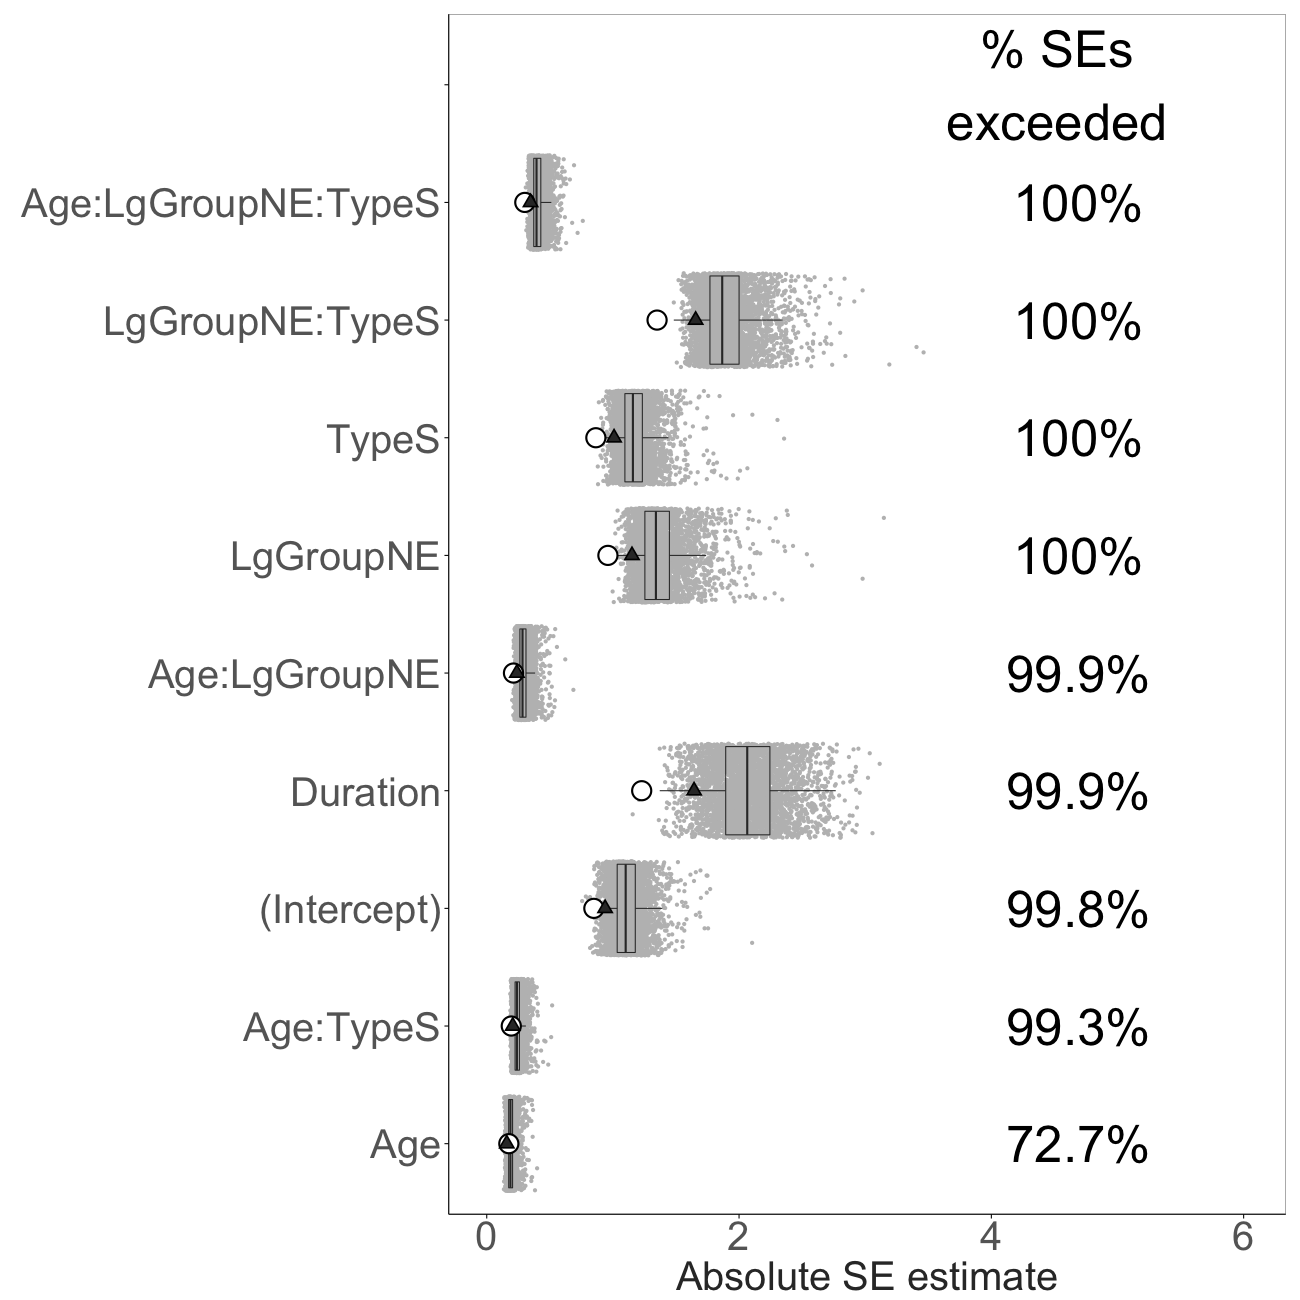
\includegraphics[width=0.44\textwidth]{figures/E1-chi-randrun-SEs-absolute.png}\label{fig:E1-ChiSEs}}
  \hfill
  \subfloat[Adults]{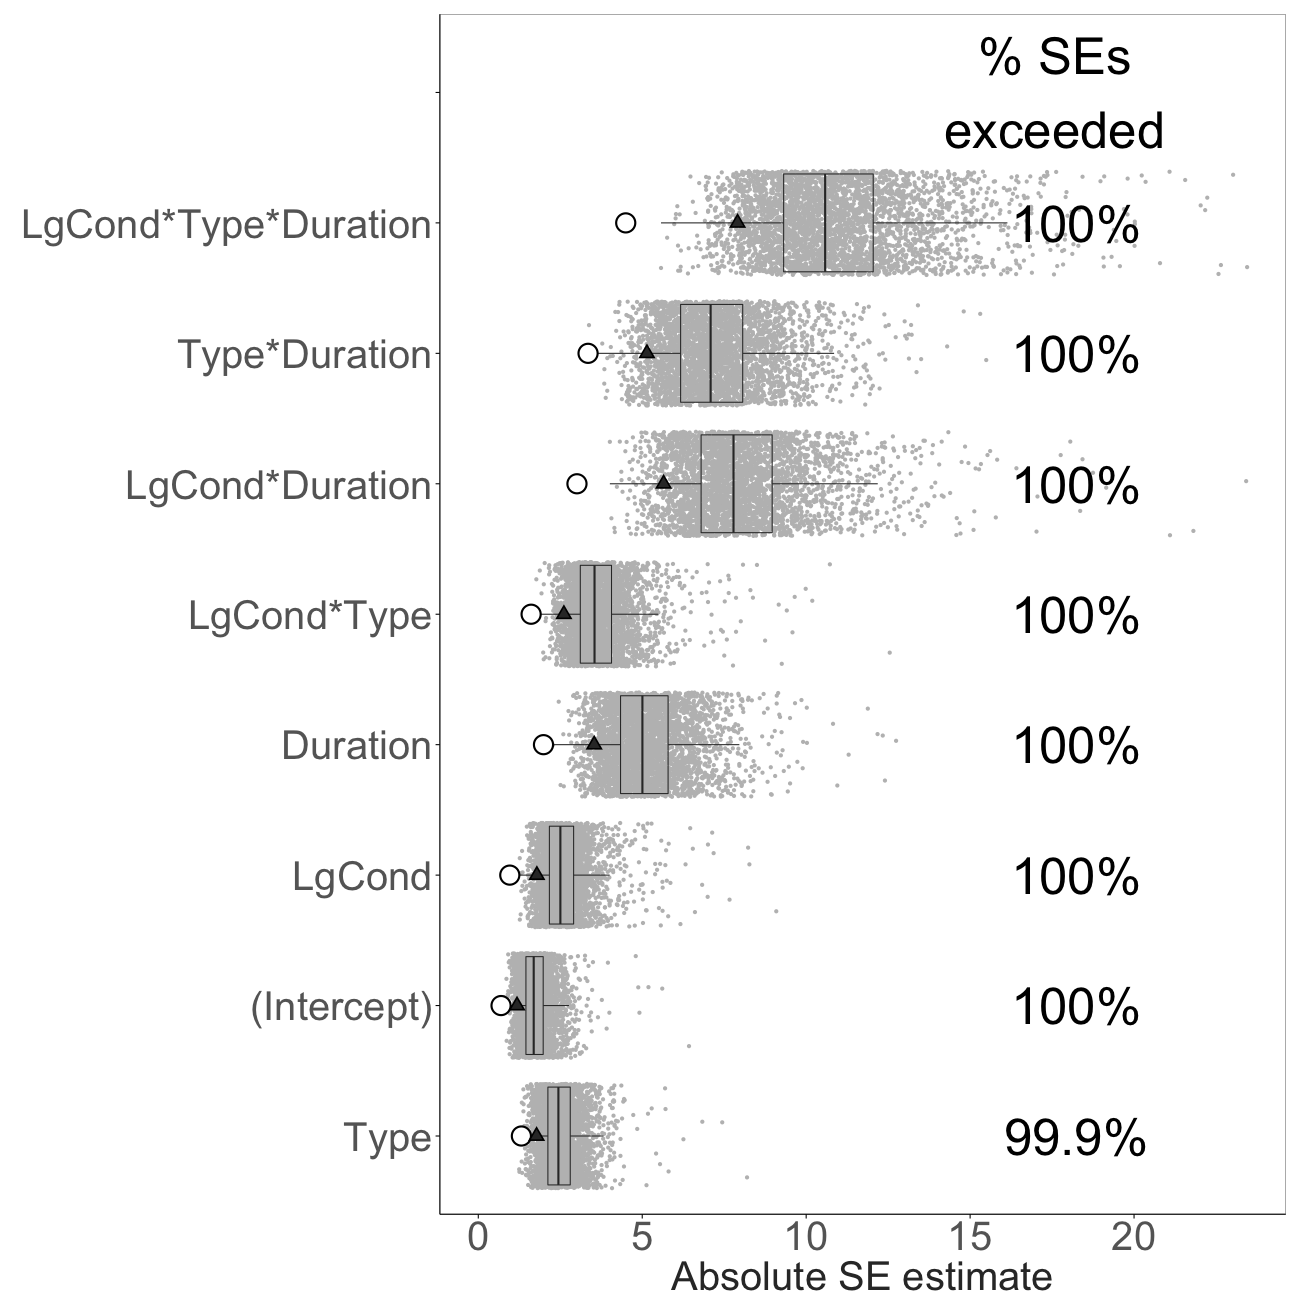
\includegraphics[width=0.44\textwidth]{figures/E1-adu-randrun-SEs-absolute.png}\label{fig:E1-AduSEs}}
  \caption{Random-permutation and original \textit{SE}-values for predictors of anticipatory gaze rates in Experiment 1.}
\label{fig:E1-SEs}
\end{sidewaysfigure}

\begin{sidewaysfigure}[!htb]
  \centering
  \textbf{Experiment 2: \textit{z} estimates}\par\medskip
  \subfloat[Children]{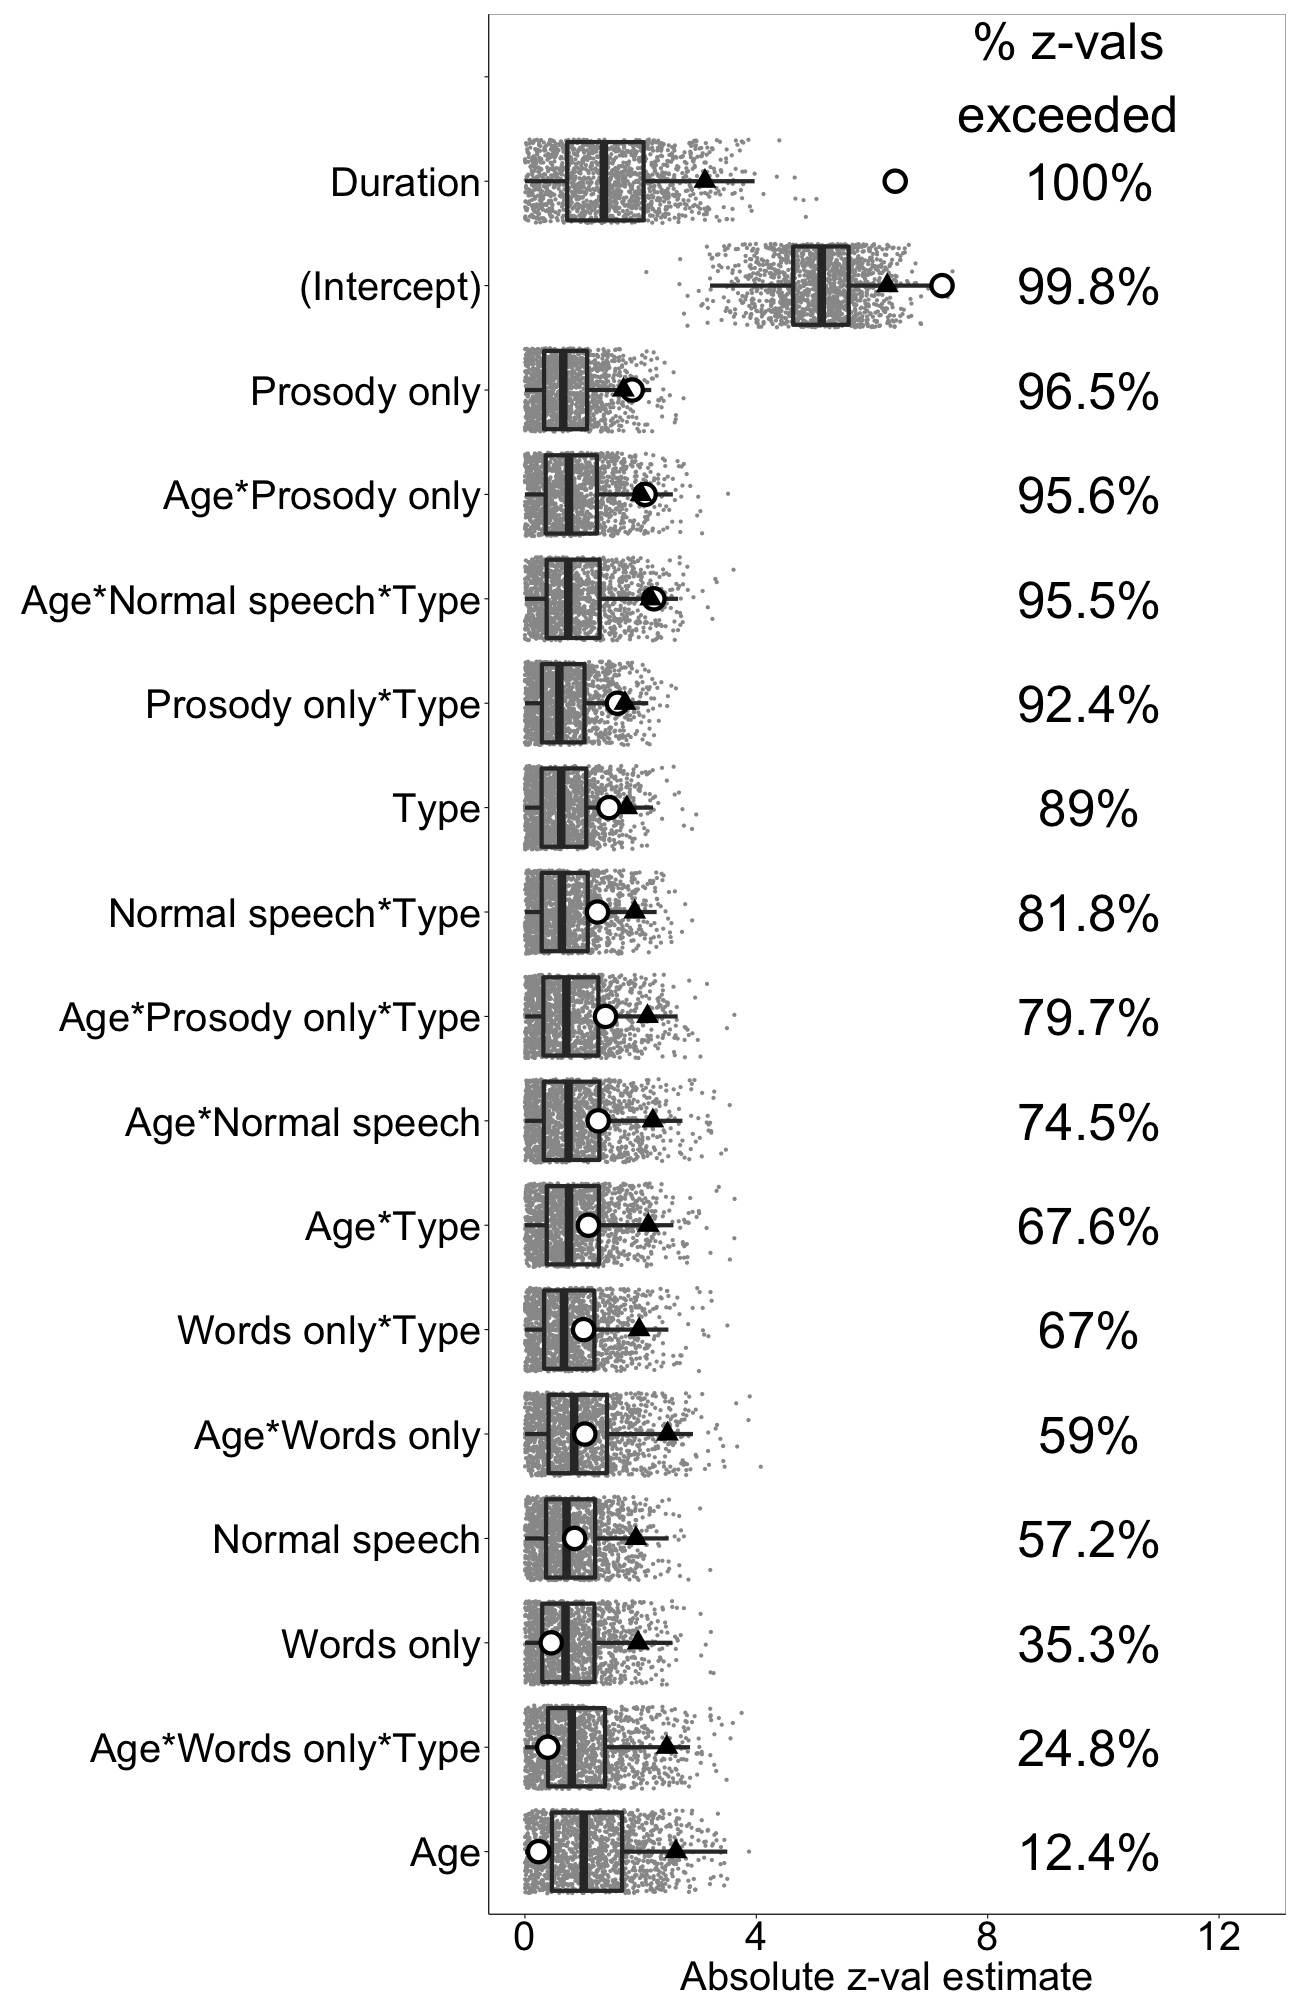
\includegraphics[width=0.44\textwidth]{figures/E2-chi-randrun-z-vals-absolute.png}\label{fig:E2-ChiTs}}
  \hfill
  \subfloat[Adults]{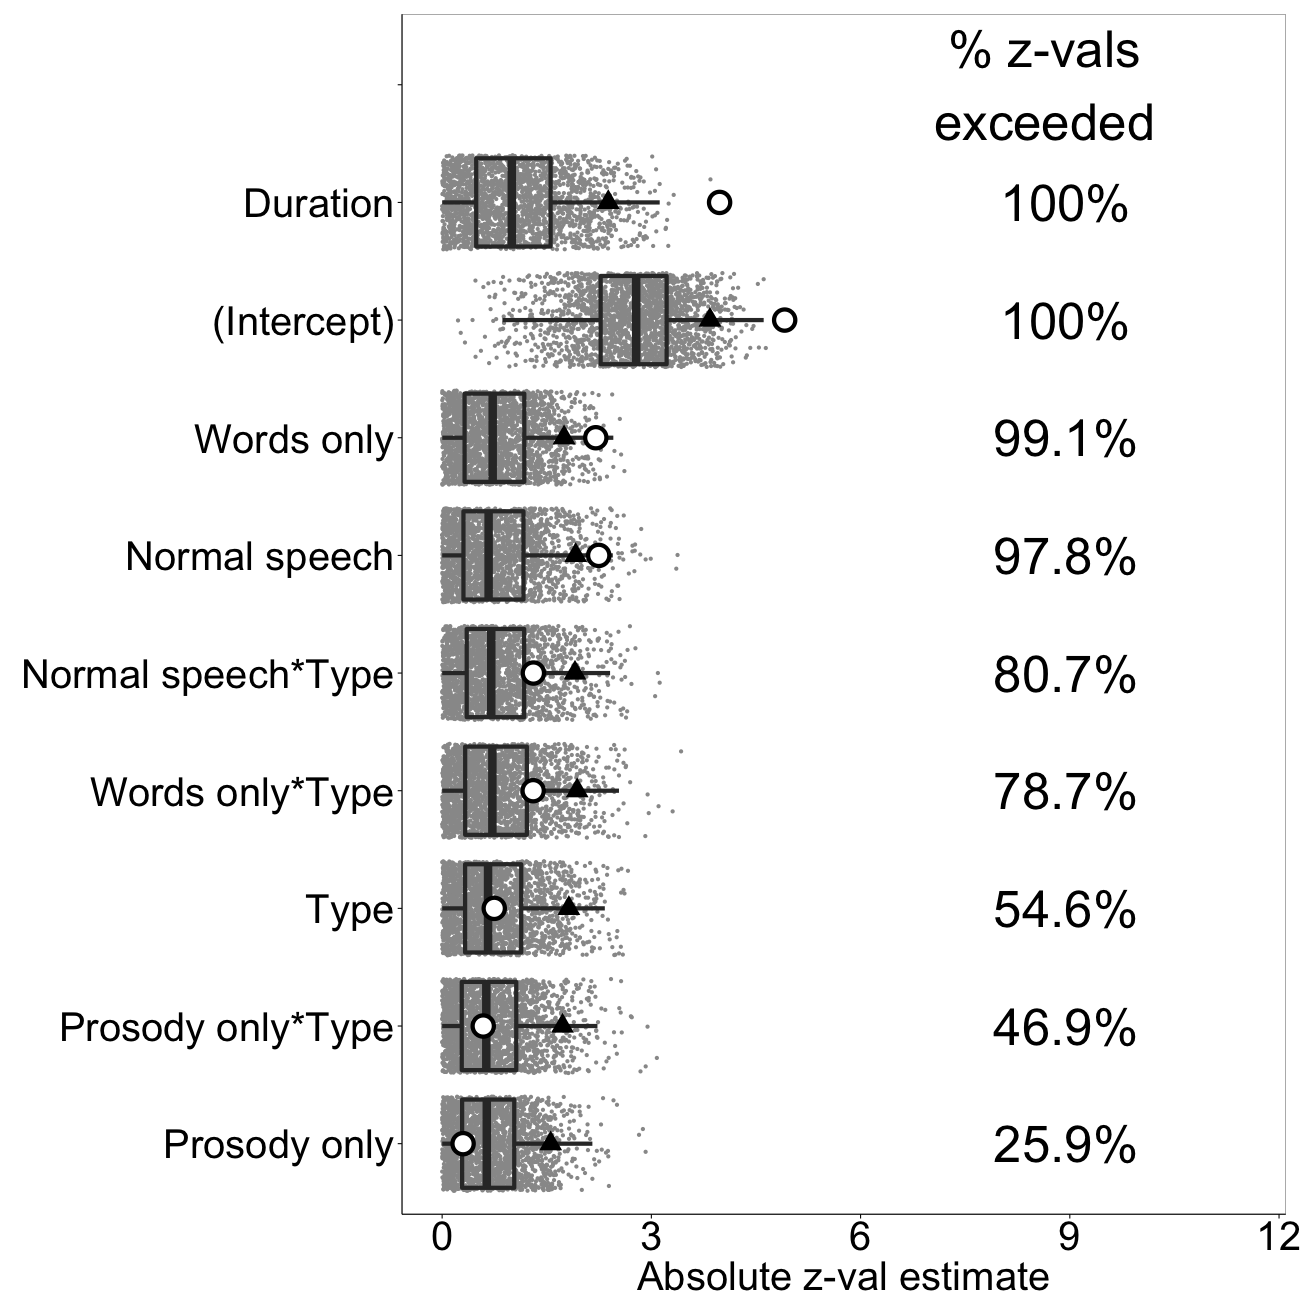
\includegraphics[width=0.44\textwidth]{figures/E2-adu-randrun-z-vals-absolute.png}\label{fig:E2-AduTs}}
  \caption{Random-permutation and original $|$\textit{z}-values$|$ for predictors of anticipatory gaze rates in Experiment 2.}
\label{fig:E2-Ts}
\end{sidewaysfigure}

\begin{sidewaysfigure}[!htb]
  \centering
  \textbf{Experiment 2: \textit{$\beta$} estimates}\par\medskip
  \subfloat[Children]{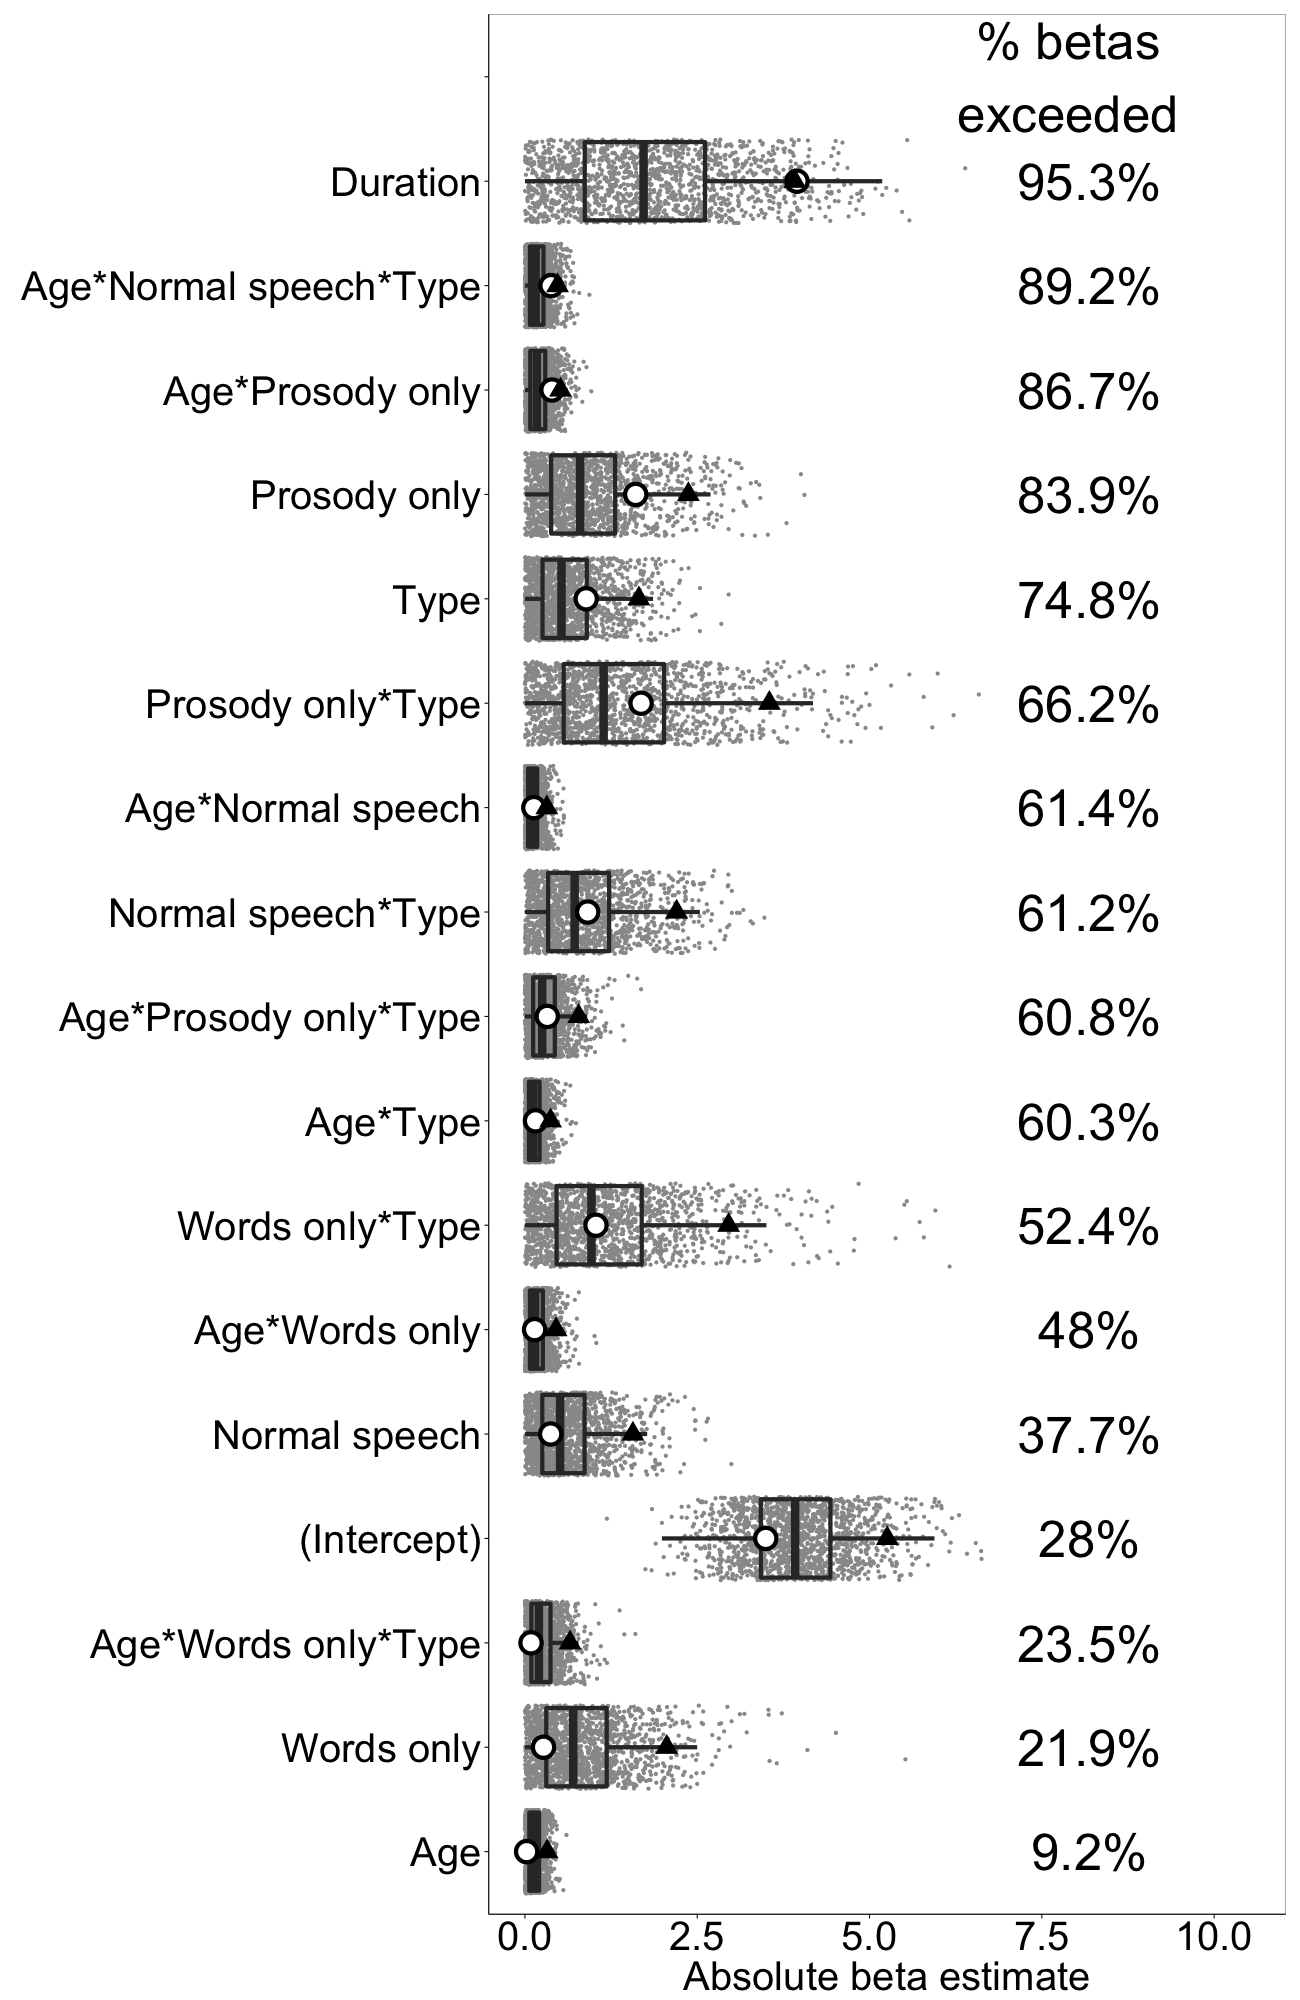
\includegraphics[width=0.44\textwidth]{figures/E2-chi-randrun-betas-absolute.png}\label{fig:E2-ChiBs}}
  \hfill
  \subfloat[Adults]{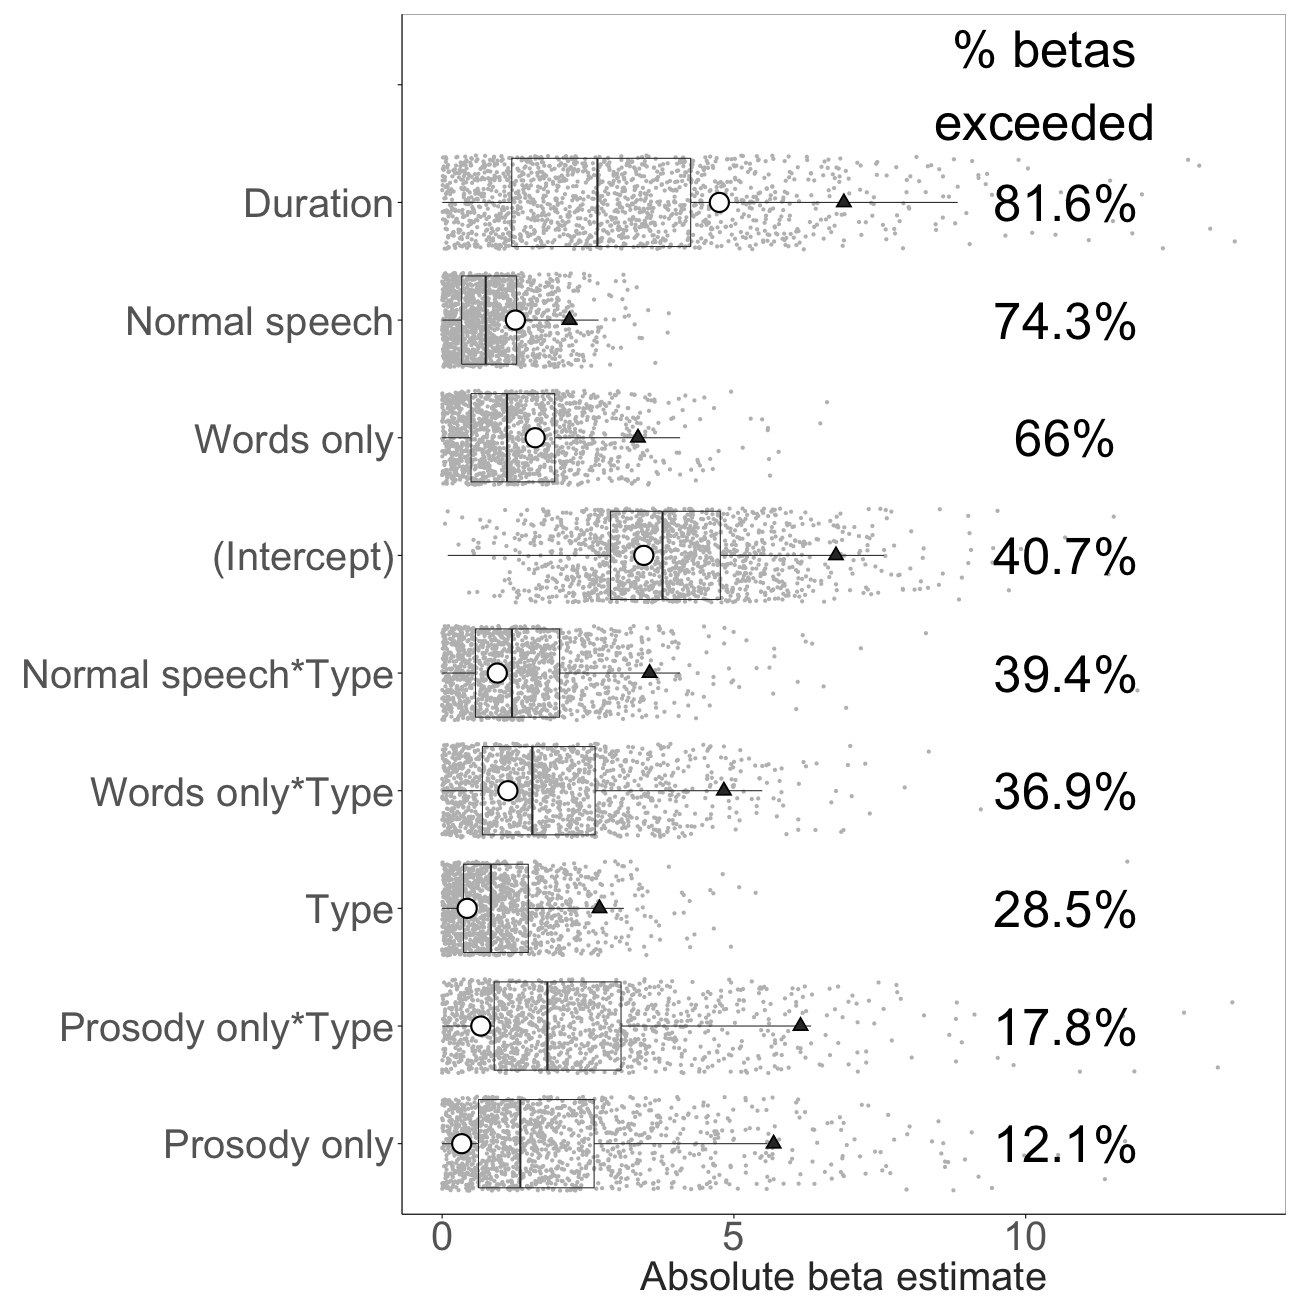
\includegraphics[width=0.44\textwidth]{figures/E2-adu-randrun-betas-absolute.png}\label{fig:E2-AduBs}}
  \caption{Random-permutation and original $|$\textit{$\beta$}-values$|$ for predictors of anticipatory gaze rates in Experiment 2.}
\label{fig:E2-Bs}
\end{sidewaysfigure}

\begin{sidewaysfigure}[!htb]
  \centering
  \textbf{Experiment 2: \textit{SE} estimates}\par\medskip
  \subfloat[Children]{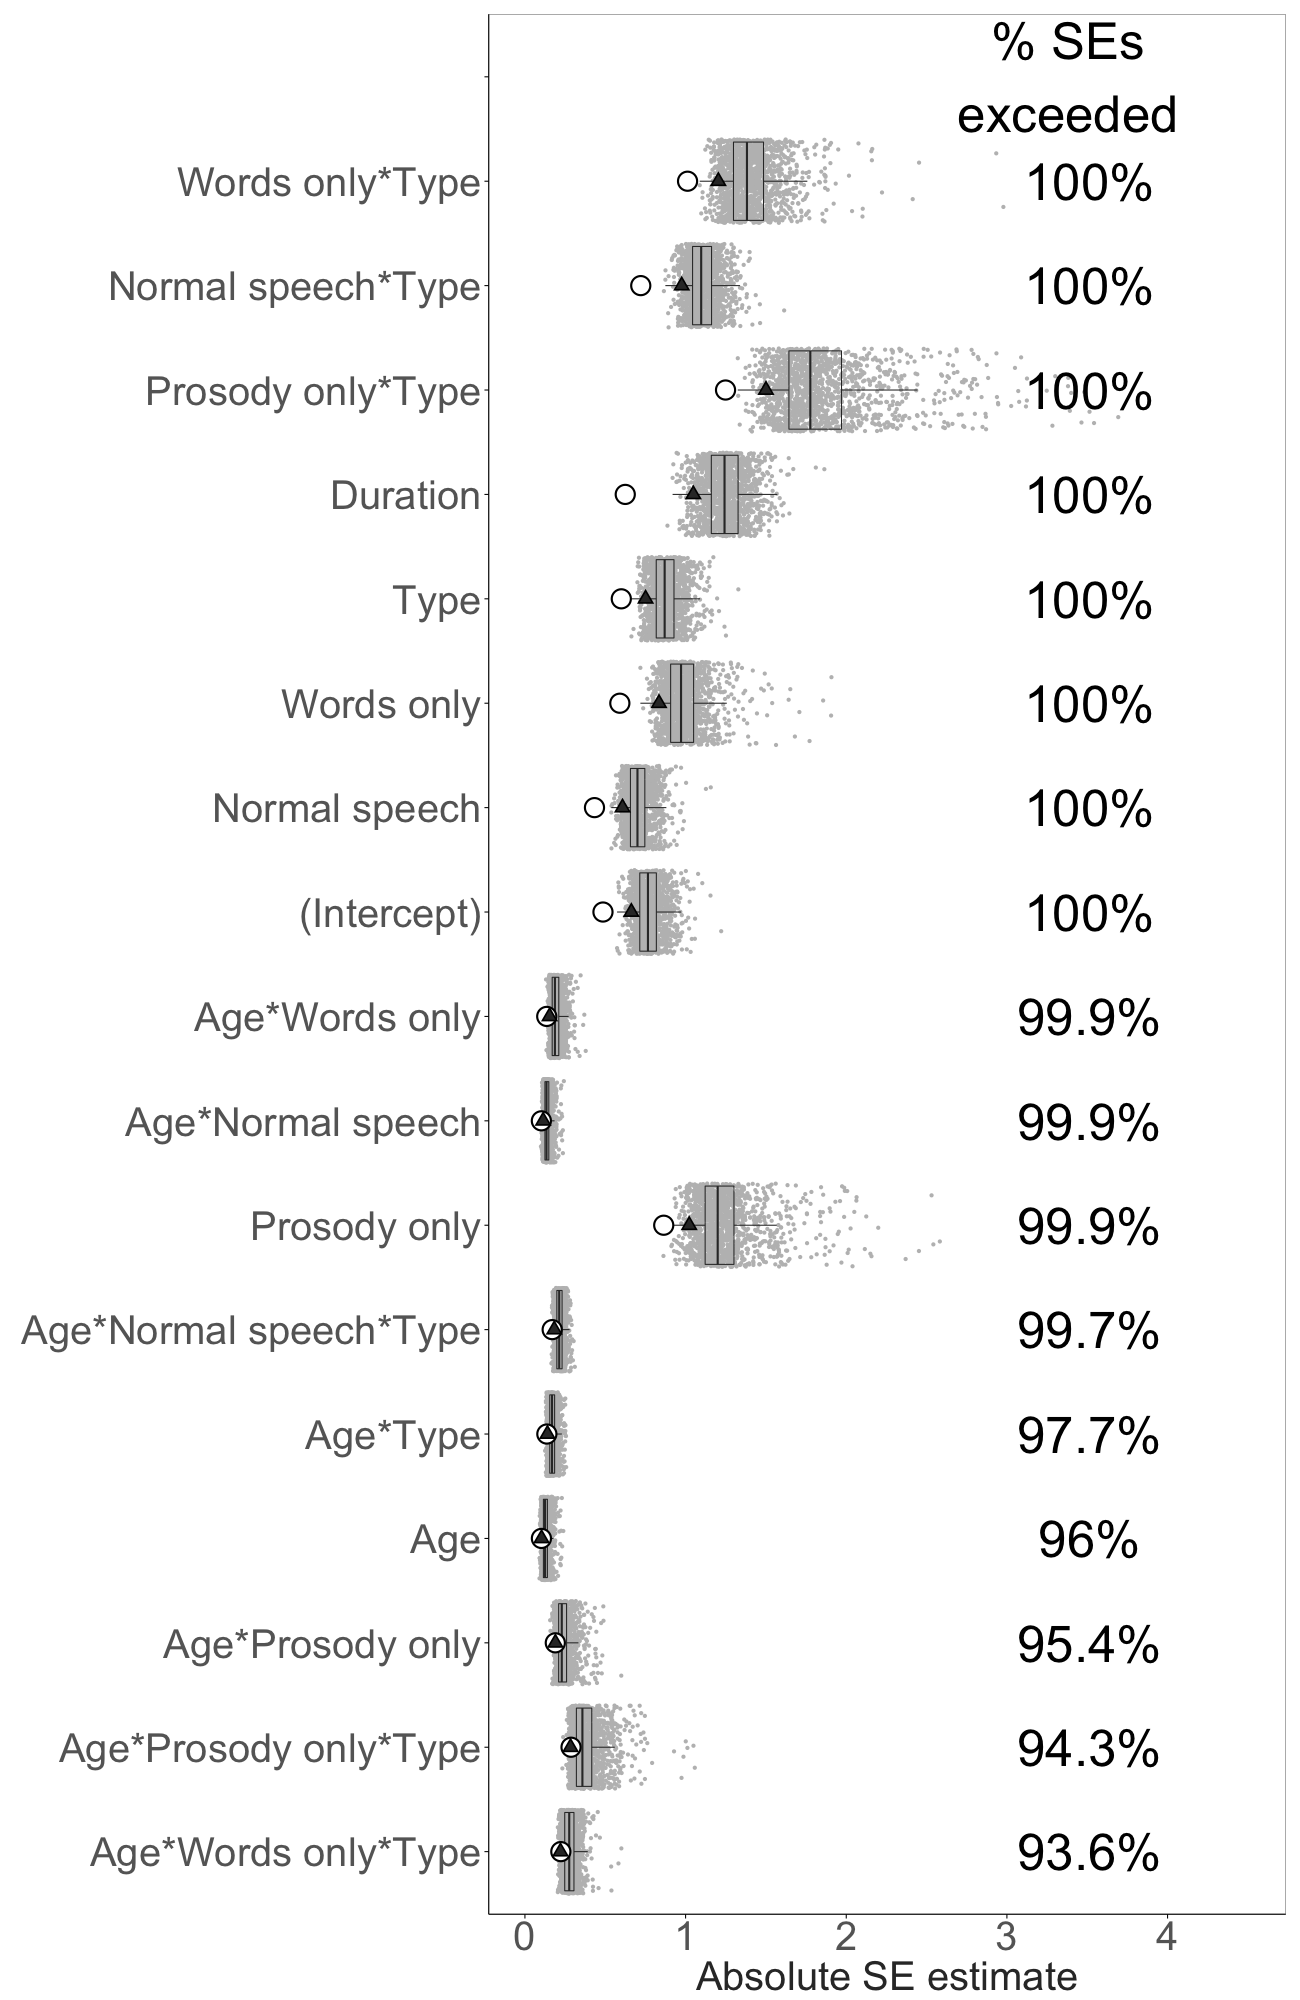
\includegraphics[width=0.44\textwidth]{figures/E2-chi-randrun-SEs-absolute.png}\label{fig:E2-ChiSEs}}
  \hfill
  \subfloat[Adults]{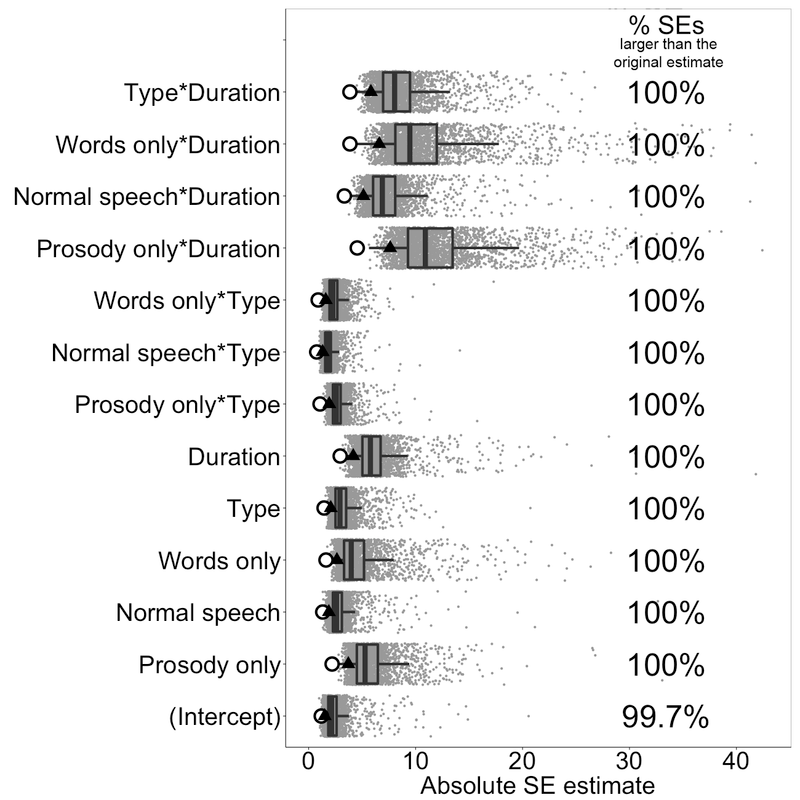
\includegraphics[width=0.44\textwidth]{figures/E2-adu-randrun-SEs-absolute.png}\label{fig:E2-AduSEs}}
  \caption{Random-permutation and original \textit{SE}-values for predictors of anticipatory gaze rates in Experiment 2.}
\label{fig:E2-SEs}
\end{sidewaysfigure}

\clearpage

\subsection{Non-convergent models}
In comparing the real and randomly permuted datasets, we excluded the output of random-permutation models that gave convergence warnings to remove erratic model estimates from our analyses. Non-convergent models made up 13--14\% of the random permutation models in Experiment 1 and 46--49\% of the random permutation models in Experiment 2. The \textit{z}-values for each predictor in the converging and non-converging models from Experiment 1 are shown in Table \ref{tab:nonconv_e1}.

Although many of the non-converging models show estimates within range of the converging models (e.g., with a mean difference of only 0.096 in median \textit{z}-value across predictors), they also show many radically outlying estimates (e.g., showing a mean difference of 146.7 in mean \textit{z}-value across predictors). Similar patterns were obtained in the non-converging models for Experiment 2 and persisted across multiple attempts with different optimizers.

We suspect that the issue derives from data sparsity in some of the random permutations. This problem is known to occur when there are limited numbers of binary observations in each of a design matrix's bins \citep{allison2004}. We could instead use zero-inflated poisson or negative binomial regression models to allow for overdispersion in our data \citep{allison2012}. However, these would give us baselines for the normal, convergent model, which is not the aim of this analysis.

\linespread{1}
\begin{sidewaystable}[!htbp]
  \begin{scriptsize}
\centering
  \begin{tabular}{lllllllllll}
    & Mean$_{C}$ & Mean$_{NC}$ & Median$_{C}$ & Median$_{NC}$ & \textit{SD}$_{C}$ & \textit{SD}$_{NC}$ & Min$_{C}$ & Min$_{NC}$ & Max$_{C}$ & Max$_{NC}$ \\
    \hline
	\textbf{\textit{Children}} &&&&& \\
    \hline
		(Intercept)			&	-1.56	&	-901.93	&	-1.59	&	-1.94	&	0.98	&	1945.68	&	-4.89	&	-11942.58	&	2.16	&	1840.2 \\
		Age					&	-0.2	&	-26.08	&	-0.21	&	-0.28	&	0.92	&	193.6	&	-4.06	&	-1151.44	&	3.57	&	751.7 \\
		LgCond				&	-0.54	&	-313.61	&	-0.56	&	-0.77	&	1.04	&	1281.84	&	-4.55	&	-7781.18	&	3.51	&	4341.3 \\
		TType				&	-0.03	&	-22.27	&	-0.03	&	0.01	&	1.05	&	1099.5	&	-3.42	&	-7137.95	&	3.56	&	5034.84 \\
		GapDur				&	0.42	&	511.04	&	0.45	&	0.61	&	1.09	&	3555.2	&	-3.86	&	-15899.54	&	3.88	&	21151.4 \\
		Age*LgCond			&	0.18	&	6.46	&	0.18	&	0.23	&	0.91	&	160.59	&	-3.35	&	-791.57		&	3.69	&	950.17 \\
		Age*TType			&	0.02	&	-7.08	&	-0.01	&	-0.05	&	0.9		&	152.2	&	-3.45	&	-815.06		&	3.43	&	741.38 \\
		LgCond*TType		&	0.18	&	-5.76	&	0.2		&	0.21	&	0.97	&	1129.35	&	-3.26	&	-6230.78	&	3.4		&	5997.59 \\
		Age*GapDur			&	-0.11	&	-24.39	&	-0.08	&	-0.12	&	0.99	&	536.89	&	-4.08	&	-2897.34	&	2.87	&	2602.11 \\
		LgCond*GapDur		&	0.22	&	475.09	&	0.2		&	0.4		&	1.12	&	2988.88	&	-3.83	&	-14231.85	&	4.02	&	17307.34 \\
		Ttype*GapDur		&	-0.02	&	-37.07	&	-0.03	&	-0.12	&	1.13	&	2824.93	&	-4.51	&	-16493.61	&	4.73	&	14994.45 \\
		Age*LgCond*TType	&	-0.1	&	-2.92	&	-0.11	&	-0.21	&	0.93	&	241.44	&	-3.34	&	-1434.96	&	3.02	&	1333.34 \\
    \hline
	\textbf{\textit{Adults}} &&&&& \\
    \hline
		(Intercept)		&	-1.85	&	-135.7	&	-1.9	&	-1.96	&	0.96	&	707.63	&	-4.48		&	-8056.34	&	1.61	&	654.56 \\
		LgCond			&	-0.35	&	-57.44	&	-0.37	&	-0.5	&	1.09	&	625.12	&	-3.8		&	-6033.9		&	3.68	&	5343.37 \\
		TType			&	-0.06	&	9.59	&	-0.06	&	0		&	1.09	&	403.93	&	-3.54		&	-4131.97	&	3.34	&	3793.07 \\
		GapDur			&	0.31	&	97.73	&	0.32	&	0.38	&	1.12	&	1159.99	&	-3.11		&	-7149.74	&	3.89	&	10669.09 \\
		LgCond*TType	&	0.18	&	31.6	&	0.18	&	0.22	&	1.03	&	560.99	&	-2.87		&	-7722.35	&	3.9		&	4377.92 \\
		LgCond*GapDur	&	0.19	&	77.34	&	0.21	&	0.18	&	1.12	&	1047.37	&	-4.18		&	-7713.96	&	3.71	&	7764.19 \\
		Ttype*GapDur	&	0		&	-50.12	&	0.01	&	-0.07	&	1.11	&	1065.37	&	-3.42		&	-10640.42	&	3.64	&	7868.74 \\
    \hline
  \end{tabular}
  \caption{Estimated \textit{z}-values for each predictor in converging (\textit{C}) and non-converging (\textit{NC}) child and adult models from Experiment 1. }
\label{tab:nonconv_e1}
 \end{scriptsize}
\end{sidewaystable}
%\linespread{2}



%\linespread{1}
%\begin{sidewaystable}[!htbp]
%  \begin{scriptsize}
%\centering
%  \begin{tabular}{lllllllllll}
%    & Mean$_{C}$ & Mean$_{NC}$ & Median$_{C}$ & Median$_{NC}$ & \textit{SD}$_{C}$ & \textit{SD}$_{NC}$ & Min$_{C}$ & Min$_{NC}$ & Max$_{C}$ & Max$_{NC}$ \\
%    \hline
%	\textbf{\textit{Children}} &&&&& \\
%    \hline
%		(Intercept)		&	-3.05	&	-2800.55	&	-3.07	&	-1496.47	&	0.84	&	3130.77		&	-5.75	&	-15569.16	&	0.26	&	-0.34 \\
%		Age			&	0.75	&	81.43		&	0.76	&	1.44		&	1.11	&	224.08		&	-3.33	&	-793.12		&	4.27	&	1094.44 \\
%		LgCond(Pros)		&	0.25	&	391.42		&	0.23	&	0.59		&	1.08	&	4135.69		&	-3.21	&	-135300.8	&	3.81	&	11272.92 \\
%		LgCond(Norm)		&	0.12	&	165.95		&	0.1	&	0.2		&	1.05	&	1544.35		&	-3.59	&	-6994.53	&	3.67	&	12125.92 \\
%		LgCond(Lex)		&	0.01	&	-320.01		&	-0.04	&	-0.33		&	1.19	&	2842.73		&	-3.37	&	-22569.54	&	4.18	&	10000.98 \\
%		TType			&	-0.37	&	-389.38		&	-0.38	&	-0.75		&	1.09	&	1832.78		&	-3.78	&	-9806.93	&	3.04	&	8548.36 \\
%		GapDur			&	0.36	&	843.66		&	0.38	&	0.74		&	1.05	&	3702.7		&	-3.52	&	-24538.48	&	3.77	&	24284.02 \\
%		Age*LgCond(Pros)	&	-0.04	&	6.36		&	-0.04	&	-0.08		&	1.06	&	551.96		&	-3.04	&	-1483.99	&	3.11	&	21619.1 \\
%		Age*LgCond(Norm)	&	-0.04	&	-15.15		&	-0.06	&	-0.2		&	1.11	&	173.55		&	-3.44	&	-816.8	&	&	3.48	&	1008.44 \\
%		Age*LgCond(Lex)		&	0.04	&	1.65		&	0.01	&	0.11		&	1.18	&	244.02		&	-3.76	&	-1406.31	&	3.86	&	1167.23 \\
%		Age*TType		&	0.04	&	2.05		&	0.03	&	0.02		&	1.09	&	204.49		&	-4.19	&	-958.44		&	3.73	&	1194.13 \\
%		LgCond(Pros)*TType	&	-0.07	&	57.09		&	-0.07	&	-0.19		&	0.96	&	3402.56		&	-3.46	&	-9987.18	&	2.89	&	132110.78 \\
%		LgCond(Norm)*TType	&	0.05	&	-0.15		&	0.06	&	0.03		&	1.01	&	1161.34		&	-4	&	-6401.71	&	3.52	&	5301.89 \\
%		LgCond(Lex)*TType	&	-0.13	&	-64.62		&	-0.12	&	-0.18		&	1.08	&	1705.68		&	-3.8	&	-9255.27	&	3.18	&	10020.13 \\
%		Age*GapDur		&	-0.21	&	-56.54		&	-0.24	&	-0.4		&	1.1	&	405.89		&	-3.73	&	-1958.19	&	3.27	&	1777.06 \\
%		LgCond(Pros)*GapDur	&	-0.14	&	-635		&	-0.12	&	-0.27		&	1.1	&	5604.19		&	-3.9	&	-26632.24	&	3.28	&	24770.67 \\
%		LgCond(Norm)*GapDur	&	0.27	&	529.45		&	0.29	&	0.48		&	1.08	&	3739.49		&	-3.37	&	-26880.55	&	3.99	&	24169.51 \\
%		LgCond(Lex)*GapDur	&	0.14	&	-378.79		&	0.19	&	0.63		&	1.19	&	68742.57	&	-4.53	&	-3282549.89	&	3.45	&	53088.85 \\
%		TType*GapDur		&	0.5	&	1361.03		&	0.5	&	0.94		&	1.13	&	4678.69		&	-2.85	&	-19023.27	&	4.3	&	28029.73 \\
%		Age*LgCond(Pros)*TType	&	-0.24	&	-68.05		&	-0.25	&	-0.38		&	1.05	&	593.7		&	-3.37	&	-21989.44	&	2.72	&	1431.64 \\
%		Age*LgCond(Norm)*TType	&	-0.11	&	-17.34		&	-0.12	&	-0.22		&	1.11	&	248.73		&	-3.78	&	-1136.43	&	3.75	&	1206.99 \\
%		Age*LgCond(Lex)*TType	&	-0.08	&	-11.56		&	-0.08	&	0		&	1.15	&	349.91		&	-3.75	&	-1565.3		&	3.85	&	1702.72 \\
%    \hline
%	\textbf{\textit{Adults}} &&&&& \\
%    \hline
%		(Intercept)		&	-1.61	&	-457.88		&	-1.72	&	-1.76	&	0.79	&	1989.16		&	-3.36	&	-43709.32	&	1.1	&	907.26 \\
%		LgCond(Pros)		&	0	&	944.53		&	-0.06	&	-0.05	&	1.01	&	43362.61	&	-2.51	&	-336814.65	&	3.45	&	1425038.89 \\
%		LgCond(Norm)		&	-0.26	&	-6.07		&	-0.23	&	-0.23	&	1	&	1160.02		&	-3.4	&	-11796.29	&	2.39	&	18948.21 \\
%		LgCond(Lex)		&	0.09	&	-4007.34	&	-0.01	&	-0.09	&	1.04	&	47289.25	&	-2.55	&	-1255648.45	&	3.3	&	186209.69 \\
%		TType			&	-0.06	&	-15.67		&	-0.06	&	-0.1	&	1.03	&	1341.86		&	-3.07	&	-17433.35	&	3.02	&	16583.07 \\
%		GapDur			&	0.37	&	216.75		&	0.43	&	0.43	&	0.97	&	2083.86		&	-2.39	&	-18593.61	&	3.06	&	27075.55 \\
%		LgCond(Pros)*TType	&	0.03	&	-705.9		&	0.11	&	0.05	&	0.96	&	26567.05	&	-3.91	&	-873190.15	&	3.03	&	75193.36 \\
%		LgCond(Norm)*TType	&	0.02	&	-70.87		&	-0.04	&	-0.03	&	1.04	&	1034.96		&	-2.66	&	-20885.3	&	3.05	&	6980.78 \\
%		LgCond(Lex)*TType	&	0.04	&	916.68		&	0.04	&	0	&	1.06	&	9636.18		&	-3.22	&	-31426.17	&	3.61	&	194241.2 \\
%		LgCond(Pros)*GapDur	&	-0.1	&	-3700.6		&	-0.12	&	-0.14	&	1.04	&	107644.13	&	-3.34	&	-3422355.79	&	2.95	&	582760.84 \\
%		LgCond(Norm)*GapDur	&	0.13	&	29469.75	&	0.11	&	0.1	&	1	&	1461329.4	&	-2.71	&	-27108.45	&	3.15	&	72670835.07 \\
%		LgCond(Lex)*GapDur	&	-0.16	&	5777.75		&	-0.12	&	-0.01	&	1.07	&	96011.19	&	-3.17	&	-1140956.82	&	2.52	&	2450843.03 \\
%		TType*GapDur		&	0.03	&	110.05		&	0.02	&	0.09	&	1.05	&	3223.11		&	-3.84	&	-44017.73	&	2.93	&	43175.22 \\
%    \hline
%  \end{tabular}
%  \caption{Estimated \textit{z}-values for each predictor in converging (\textit{C}) and non-converging (\textit{NC}) child and adult models from Experiment 2. }
%\label{tab:nonconv_e2}
% \end{scriptsize}
%\end{sidewaystable}
%%\linespread{2}




\section{Pairwise developmental tests}
\label{sec:pairwisedev}
\setcounter{figure}{0}
Experiments 1 and 2 both showed effects of age in interaction with linguistic condition and transition type. To explore these effects in more depth, in each permutation we recorded the average difference score for each participant, for each predictor that interacted with age (e.g., English minus non-English anticipatory switches for each participant). We then used these values to compute an average difference score over the participants in each age group (e.g., age 3, 4, and 5) within each random permutation. This averaging process produces 5,000 baseline-derived difference scores for each age group.

We then made pairwise age comparisons of the difference scores (e.g., the linguistic condition effect in 3-year-olds vs. 4-year-olds), computing the percent of random-permutation difference scores exceeded by the real-data difference score. If the real-data difference score exceeded 95\% of the random-data age difference scores, we deemed it to be an age effect significantly different from chance, e.g., a significant difference between ages three and four in the effect of linguistic condition. This procedure is essentially a two-tailed \textit{t}-test, adapted for use with the randomly permuted baseline data.

In each of the plots below, the black dot represents the real data value for the effect being shown (the difference score). The effect sizes from the 5,000 randomly permuted data sets are shown as a distribution. The percentage displayed is the percentage of random permutation difference scores exceeded by the original data differences score (taking the absolute value of all data points for a two-tailed test). Comparisons marked with 95\% or higher are significant at the \textit{p}$<$0.05 level.

\begin{sidewaysfigure}[!htb]
\begin{center}
\textbf{Experiment 1: Age and linguistic condition}\par\medskip
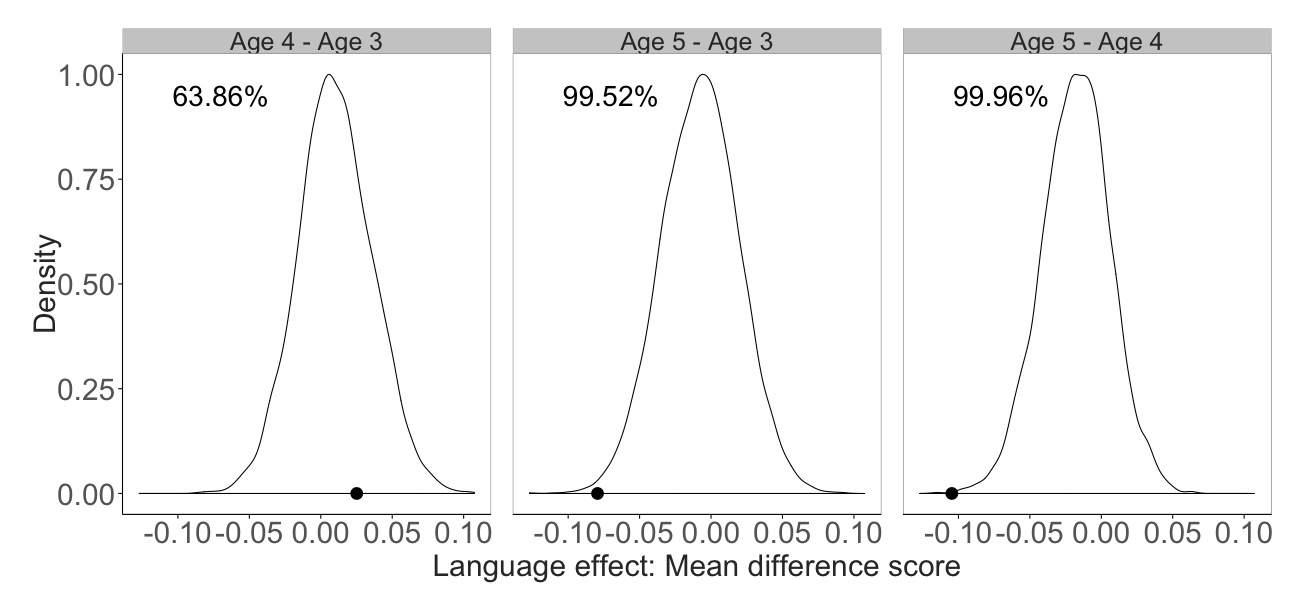
\includegraphics[width=0.95\textwidth]{figures/E1-child-randvsreal-ttest-agebylg.png}
\end{center}
\caption{Pairwise comparisons of the language condition effect across ages in Experiment 1.}
\label{fig:E1-lgageinteraction}
\end{sidewaysfigure}

\begin{sidewaysfigure}[!htb]
\begin{center}
\textbf{Experiment 2: Age and the \textit{prosody only} condition}\par\medskip
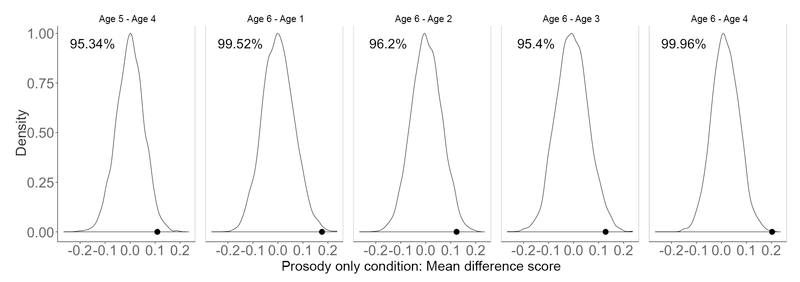
\includegraphics[width=0.95\textwidth]{figures/E2-child-randvsreal-ttest-muffledages.png}
\end{center}
\caption{Significant pairwise comparisons of the \textit{prosody only}-\textit{no speech} linguisitic condition effect, across ages in Experiment 2. Non-significant comparisons are not shown.}
\label{fig:E2-lgageinteraction}
\end{sidewaysfigure}

\begin{sidewaysfigure}[!htb]
\begin{center}
\textbf{Experiment 2: Age, transition type, and \textit{normal} speech}\par\medskip
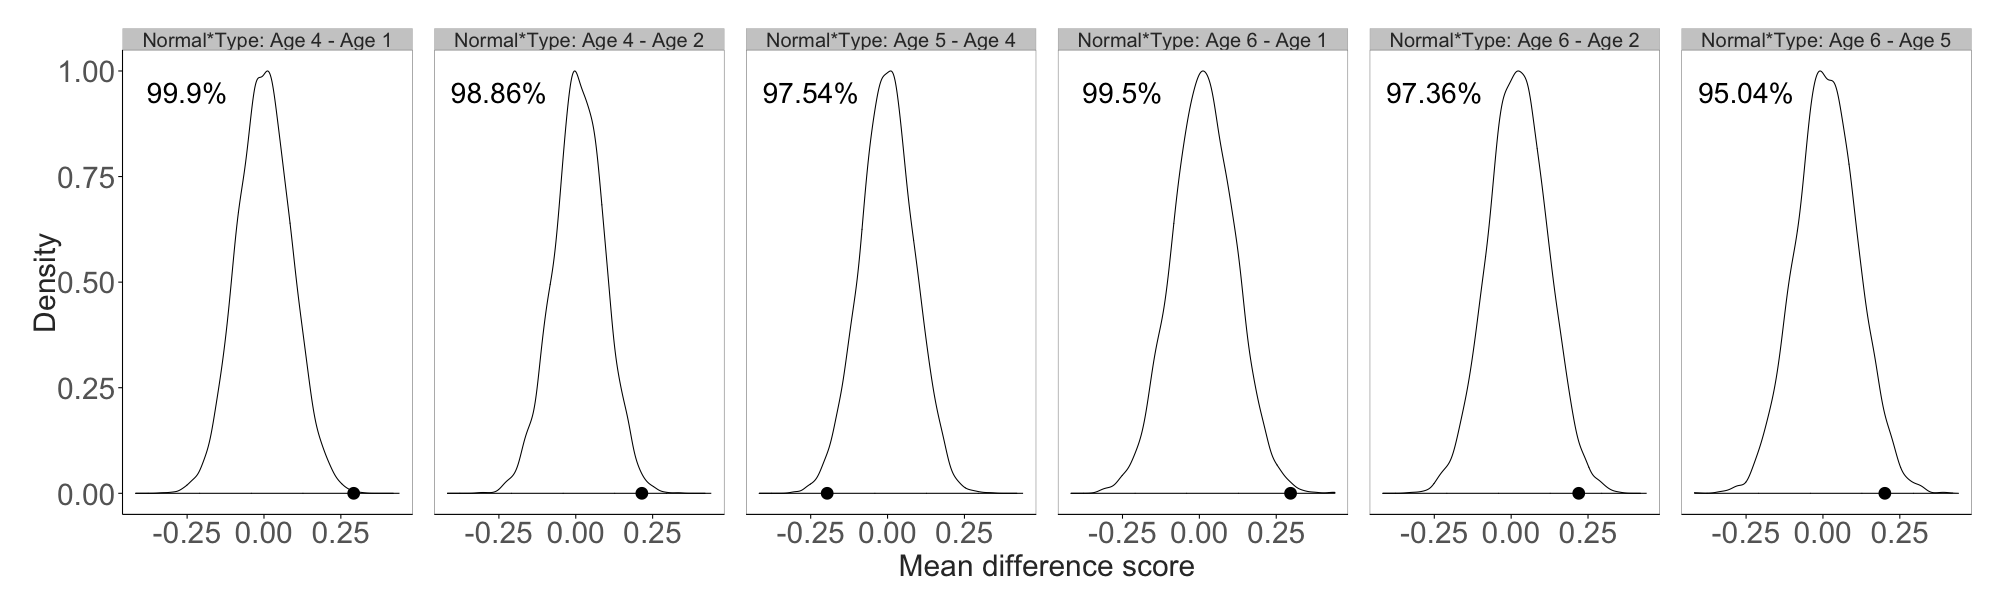
\includegraphics[width=0.95\textwidth]{figures/E2-child-randvsreal-ttest-normaltypesages.png}
\end{center}
\caption{Significant pairwise comparisons of the \textit{normal speech}-\textit{no speech} language condition effect for transition type, across ages, in Experiment 2. Non-significant comparisons are not shown.}
\label{fig:E2-lgagetypeinteraction}
\end{sidewaysfigure}

\section{Boredom-driven anticipatory looking}
\label{sec:boredlooks}
\setcounter{figure}{0}

One alternative hypothesis for children's anticipatory gazes is that they look at the current speaker at the start of each turn, but then grow bored and start looking away at a constant rate. Even though this alternative hypothesis does not predict the primary effects in our data (e.g., the difference between questions and non-questions), we cannot rule out the possibility that a portion of participants' saccades come from boredom.

The data plotted here show a hypothetical group of boredom-driven participants (gray dots) and participants from the actual data in Experiment 2 (black dots). The hypothetical boredom-driven participants look away from the current speaker at a linear rate, beginning one second after the start of a turn.

\begin{figure}[!htb]
\begin{center}
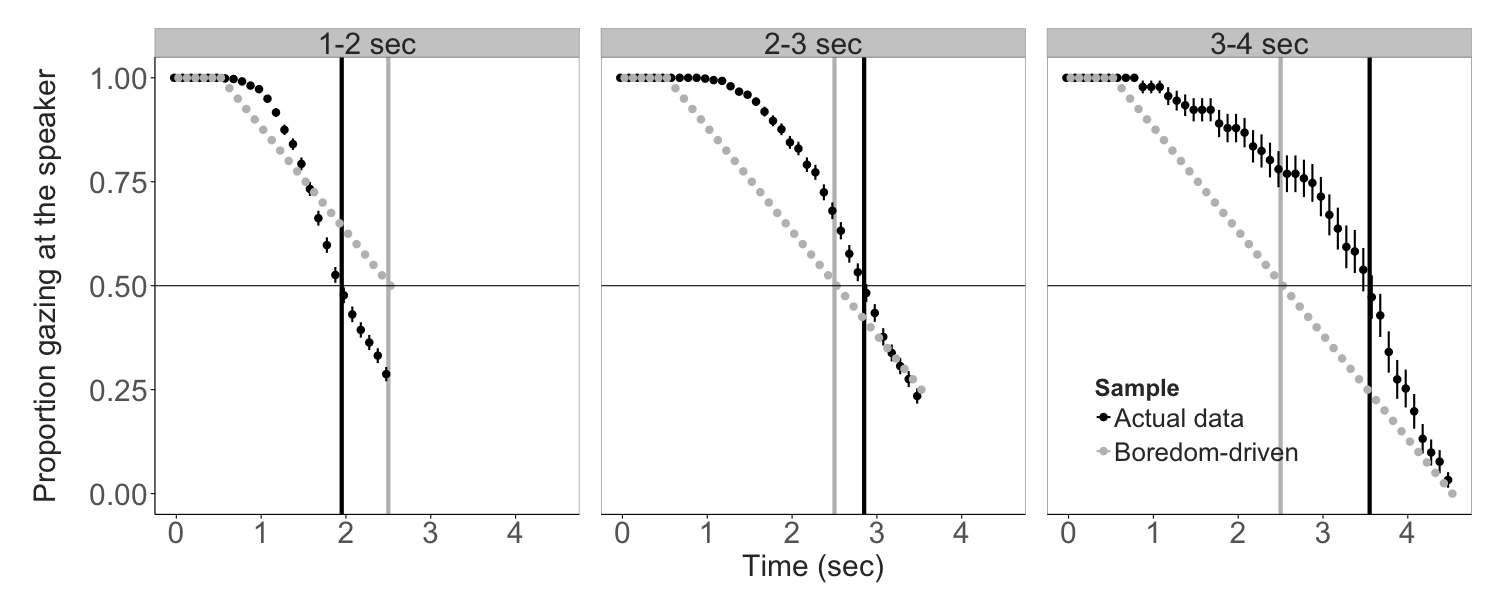
\includegraphics[width=0.95\textwidth]{figures/boredom-hypothesis.png}
\end{center}
\caption{Proportion of participants (hypothetical boredom-driven$=$gray; actual Experiment 2$=$black) looking at the current speaker, split by turn duration. Vertical bars indicate standard error in the experimental data.}
\label{fig:boredomhypothesis}
\end{figure}

If children's switches away from the current speaker were purely driven by boredom, they would switch away equally quickly on long and short turns. Therefore, their crossover point---the point in time at which 50\% of the children have switched away from the current speaker---would be the same for all turns, no matter the length of the turn. This pattern is demonstrated in the hypothetical boredom-driven crossover points, which always occur 2.5 seconds after the start of speech (gray vertical lines; Figure \ref{fig:boredomhypothesis}).

In children's \textit{actual} looking data we see that crossover points increase with turn duration: 2.0, 2.9, and 3.6 seconds after the start of speech for turns with durations of 1--2, 2--3, and 3--4 seconds, respectively (black vertical lines; Figure \ref{fig:boredomhypothesis}). This pattern suggests that, though children do look away as the turn is unfolding, their looks away are not simply driven by boredom.

Are the looks away in Figure \ref{fig:boredomhypothesis} still too early to count as ``turn-transition'' anticipation? It is true that children start looking away after one second has passed, but then only gradually. Some of these early looks away may be boredom-driven, but it is equally plausible that some of them are turn-driven. Early predictive behavior is common in turn-taking studies with adults, in both constrained turn-taking tasks \citep{de-ruiter2006, gisladottir2015, bogelstorreira2015} and in spontaneous conversation \citep{holler2015, bogels2015}. Although this same pattern has yet to be established for children's turn predictions, the looking behavior here is at least consistent with adult response patterns in previous work. Additionally, because our analysis windows in the main study only overlapped with the pre-gap utterance by 300 msec (Main paper; Figure 2), our primary results are unlikely to capture any of these very early or early boredom-driven gaze switches, which makes them unproblematic either way in the current analysis.

We therefore conclude that the boredom-driven effects in our data are unlikely to change our primary results, though we acknowledge that characterizing different gaze switching strategies in this kind of data is an important avenue for future work.

\clearpage

\section{Puppet pair and linguistic condition}
\label{sec:puppetconfound}
\setcounter{figure}{0}
The design for Experiment 2 does not fully cross puppet pair (e.g., robots, blue puppets) with linguistic condition (e.g., \textit{words only} and \textit{no speech}). Even though each puppet pair is associated with different conversation clips across children (e.g., robots talking about kitties, birthday parties, and pancakes), the robot puppets themselves were exclusively associated with the \textit{words only} condition. Similarly, merpeople were exclusively associated with \textit{prosody only} speech, and the puppets wearing dressy clothes were exclusively associated with the \textit{no speech} condition. We designed the experiment this way to increase its pragmatic felicity for older children (i.e., robots make robot sounds, merpeople's voices are muffled under the water, the party-going puppets are in a `party' room with many other voices). There is therefore a confound between linguistic condition and puppet pair; for example, children could have made fewer anticipatory switches in the \textit{prosody only} condition because the puppets were less interesting. To test whether puppet pair drove the condition-based differences found in Experiment 2, we ran a follow-up study.

\medskip
\noindent \textbf{Methods}
\medskip

\noindent We recruited 30 children between ages 3;0 and 5;11 from the Children's Discovery Museum of San Jose, California to participate in our experiment. All participants were native English speakers. Children were randomly assigned to one of six videos (five children per video).

\medskip
\noindent \textit{Materials}. We created 6 short videos from the stimulus recordings made for Experiment 2. Each video featured a puppet pair (red/blue/yellow/robot/ merpeople/party-goer; Main paper; Figure 5). Puppets in all six videos performed the exact same conversation recording (`birthday party'; Experiment 2) with normal, unmanipulated speech. This experiment therefore holds all things constant across stimuli except for the appearance of the puppets.

\medskip
\noindent \textit{Procedure}. We used the same experimental apparatus and procedure as in Experiments 1 and 2. Each participant was randomly assigned to watch only one of the six puppet videos. Five children watched each video. As in Experiment 2, the experimenter immediately began each session with calibration and then stimulus presentation because no special instructions were required. The entire experiment took less than three minutes.

\medskip
\noindent \textit{Data preparation}. We identified anticipatory gaze switches to the upcoming speaker using the same method as in Experiments 1 and 2.

\bigskip
\noindent \textbf{Results and discussion}
\medskip

\noindent We modeled children's anticipatory switches (yes or no at each transition) with mixed effects logistic regression, including puppet pair (robots/mer- people/party-goers/other-3) as a fixed effect and participant and turn transition as random effects. We grouped the red, blue, and yellow puppets together because they collectively represented the puppets used in the \textit{normal} speech condition---this follow-up experiment is meant to test whether the condition-based differences from Experiment 2 arose from the puppets used in each condition.

\begin{figure}[!htb]
\begin{center}
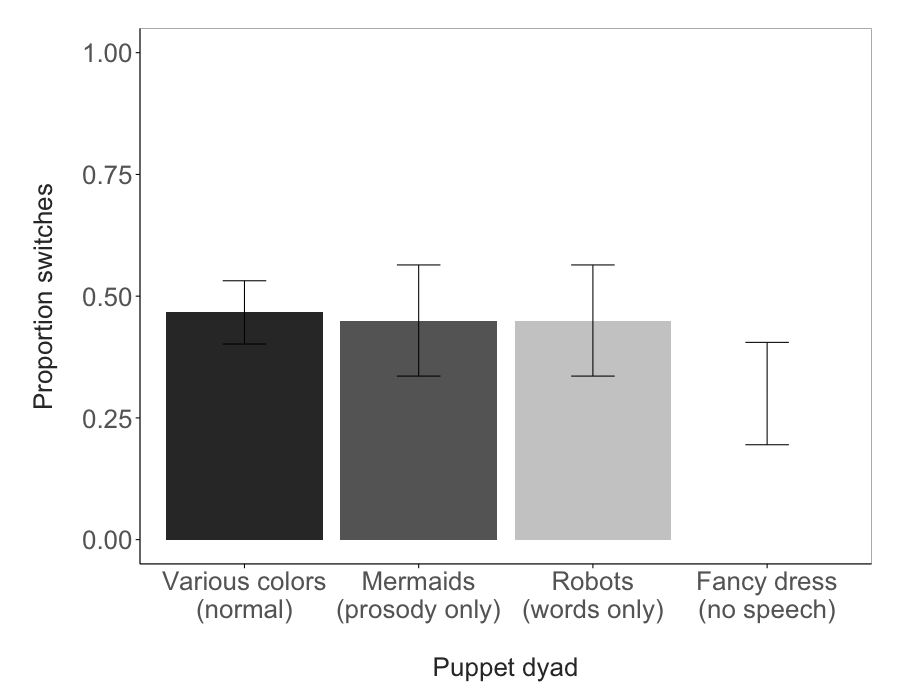
\includegraphics[width=0.95\textwidth]{figures/all-puppetdyads-bars.png}
\end{center}
\caption{Proportion gaze switches across puppet pairs when linguistic condition and conversation are held constant.}
\label{fig:pairconfound}
\end{figure}

\clearpage

\linespread{1}
\begin{table}
\begin{center}
  \begin{tabular}{llcccc}
%    \hline
           &  Estimate & Std. Error & \textit{z} value & Pr($>$$|$\textit{z}$|$) \\
    \hline
		 \footnotesize{\textit{Reference level: normal-condition puppets}} &&&& \\
    \hline
     (Intercept) 							& -0.148	& 0.328		& -0.451		& 0.652 \\
     Puppets$=$\textit{mermaid} 	& -0.076	& 0.655		& -0.116		& 0.908 \\
     Puppets$=$\textit{robot} 		& -0.071	& 0.653		& -0.109		& 0.913 \\
     Puppets$=$\textit{party} 		& -0.782	& 0.687		& -1.138		& 0.255 \\
    \hline
		 \footnotesize{\textit{Reference level: mer-puppets}} &&&& \\
    \hline
     (Intercept) 							& -0.224	& 0.568		& -0.394		& 0.694 \\
     Puppets$=$\textit{robot} 		& 0.0048	& 0.801		& 0.006			& 0.995 \\
     Puppets$=$\textit{party} 		& -0.706	& 0.827		& -0.854		& 0.393 \\
    \hline
		 \footnotesize{\textit{Reference level: robot puppets}} &&&& \\
    \hline
     (Intercept) 							& -0.219	& 0.566		& -0.387		& 0.699 \\
     Puppets$=$\textit{party} 		& -0.711	& 0.827		& -0.860		& 0.390 \\
    \hline
		 \footnotesize{\textit{Reference level: party-goer puppets}} &&&& \\
    \hline
     (Intercept) 							& -0.93		& 0.607		& -1.533		& 0.125 \\
  \end{tabular}
\end{center}
  \caption{Model output for children's anticipatory gaze switches with reference levels varied to show all possible pairwise differences between puppet pairs.}
\label{tab:control_exp}
\end{table}
%\linespread{2}

In four versions of this model, we systematically varied the reference level of the puppet pair to check for any cross-condition differences. We found no significant effects of puppet pair on switching rate (all \textit{p}$>$0.25; Table \ref{tab:control_exp}).

We take this finding as evidence that our decision to not fully cross puppet pairs and linguistic conditions in Experiment 2 was unlikely to have affected children's anticipatory gaze rates above and beyond the intended effects of linguistic condition.

\newpage

\bibliographystyle{model5-names}
\biboptions{authoryear}
\bibliography{anticip}
\clearpage

\end{document}
